\documentclass[3p]{elsarticle}
%\documentclass[review]{elsarticle}

\usepackage{lineno,hyperref}

\usepackage{amsmath, amsfonts, amsthm, mathrsfs, bm, bbm}
\usepackage{siunitx} \sisetup{retain-zero-exponent}
\usepackage{standalone}
\usepackage{tikz}
\usetikzlibrary{matrix, chains, backgrounds, calc, shapes, arrows, arrows.meta, fit, positioning}
\usepackage{pgfplots, pgfplotstable}
\usepackage{xcolor}
\usepackage{subcaption}
\captionsetup[subfigure]{labelformat = parens, labelsep = space, font = small}

\modulolinenumbers[5]

\journal{Computer Methods in Applied Mechanics and Engineering.}

\bibliographystyle{elsarticle-num}

\newcommand{\sputnik}{{\ttfamily \fontseries{b}\selectfont SPUTNIK }}
\newcommand{\micro}{{\ttfamily \fontseries{b}\selectfont MICRO }}
\newcommand{\fe}{FE$^2$}

%--------------------------------------------------

\begin{document}

\begin{frontmatter}

\title{Linear and modal analysis applying the FE$^2$ multi-scale method for composite materials.}

%\author{Elsevier\fnref{myfootnote}}
%\fntext[myfootnote]{Since 1880.}
%\address{Carrer Jordi Girona 29, Barcelona}
\author[bsc]{Guido Giuntoli}
\author[bsc]{Mariano V\'azquez}
\author[upc]{Sergio Oller}
\address[bsc]{Barcelona Supercomputing Center, Barcelona, Spain}
\address[upc]{Universitat Polit\`ecnica de Catalunya, Barcelona, Spain}

%---------------------------------------------------------------------------------------------------

\begin{abstract}
We study the homogenization method with \emph{uniform strains} boundary
conditions in 2D composite material problems.
We assume linear materials and small deformations approach.
Two examples are solved including both: a linear response calculation (force
\emph{vs.} displacement relation) and a modal calculation of the eigenvalues 
of the system, the last ones are directly related with the natural oscillations 
frequencies of the system.
All the problems are compared with the micro-model and with other homogenization 
theories such as the parallel and serial rule of mixtures.
A detail explanation about the computational implementation of the algorithm using 
the finite element method is given.
\end{abstract}

\begin{keyword}
homogenization \sep composite materials 
\MSC[2010] 00-01\sep  99-00
\end{keyword}
 
\end{frontmatter}

%\linenumbers

%---------------------------------------------------------------------------------------------------
\section{Introduction}

The increasing demand in the using of composite materials in industry inspired people
to get a deeper understanding of the physical behavior of them. By this way it
can be possible to design not only the structure itself but also the material's
micro-structure allowing a cheaper and faster design and more secure structures.

There are several techniques used to model solid composite structures and the
most used are based on the finite elements method (FEM).
The simplest idea is to use the \emph{brute force method}
even called \emph{micro-model}, this means to solve the problem with FEM
taking into account the smallest heterogeneities that the material has.
This generally ends in high computational cost problem and in very difficult mesh
generation problem depending on the micro-structure, specially if it is non
periodic.

Lot of theories have been developed since the 50th decade for trying to solve
the problem. We are going to focused on a FE$^2$ theory based on
\emph{uniform strains} boundary conditions that has proved to be a very accurate technique.
Our objective is to measure the accuracy of this numerical method on the linear 
range through out solving two examples and comparing the results with the 
\emph{micro-model} method and other theories such as the \emph{parallel mixture} 
and \emph{serial mixture} rules. 

In the first part of this work we describe the basics on multi-scale methods
for composite material calculations providing a detailed description of the
numerical implementation used. We describe two kinds of calculations: a simple
linear analysis, i.e., the force \emph{vs.} displacement relation
and a modal analysis that allows to obtain the natural oscillations
frequencies.
In the other part we solve two 2D problems with linear materials using this 
homogenization procedure and we compare the solution with the \emph{micro-model} 
and the \emph{parallel} and \emph{serial mixture} rules. 

%---------------------------------------------------------------------------------------------------

\section{The \fe multi-scale method}

The idea of homogenization methods is to get average properties of the physical
quantities in finite portions of the domain. With these properties, then, is 
possible to replace the heterogeneous structure with an equivalent homogeneous
one reducing the calculation complexity. This allows to the so called
\emph{multi-scale} methods where the problem is separated into two (or more)
scales and different calculations are done in the both scales
for obtaining the solution. Here we aimed our study only to two scale problems
which are enough to solve most of the composite material problems.

The description of the multi-scale theory exposed here and the 
notation was based on the works of Miehe \cite{miehe2002}.

This method is aimed to get and accurate representation of the displacement 
and stress fields inside a structure made of composite materials, microscopically
they look like a periodic pattern of different homogeneous materials.

The method is based on representing the macroscopic structure as a one made of 
homogeneous material where the constitutive properties will be calculated as an 
average of the properties inside a \emph{representative volume element} (\emph{r.v.e.}),
see Fig.~\ref{fig:multi-scale}, where 
$\overline{\bm{u}}, \overline{\bm{\epsilon}}, \overline{\bm{\sigma}}$
represents the displacement, strain and stress fields on the homogenized
macro-structure respectively and
${\bm{u}}, {\bm{\epsilon}}, {\bm{\sigma}}$
represents the displacement, strain and stress fields on the \emph{r.v.e.}.

% <figure multi-scale scheme>
\begin{figure}[!ht]
\centering
\resizebox{8cm}{!}{\documentclass{standalone}

\begin{document}

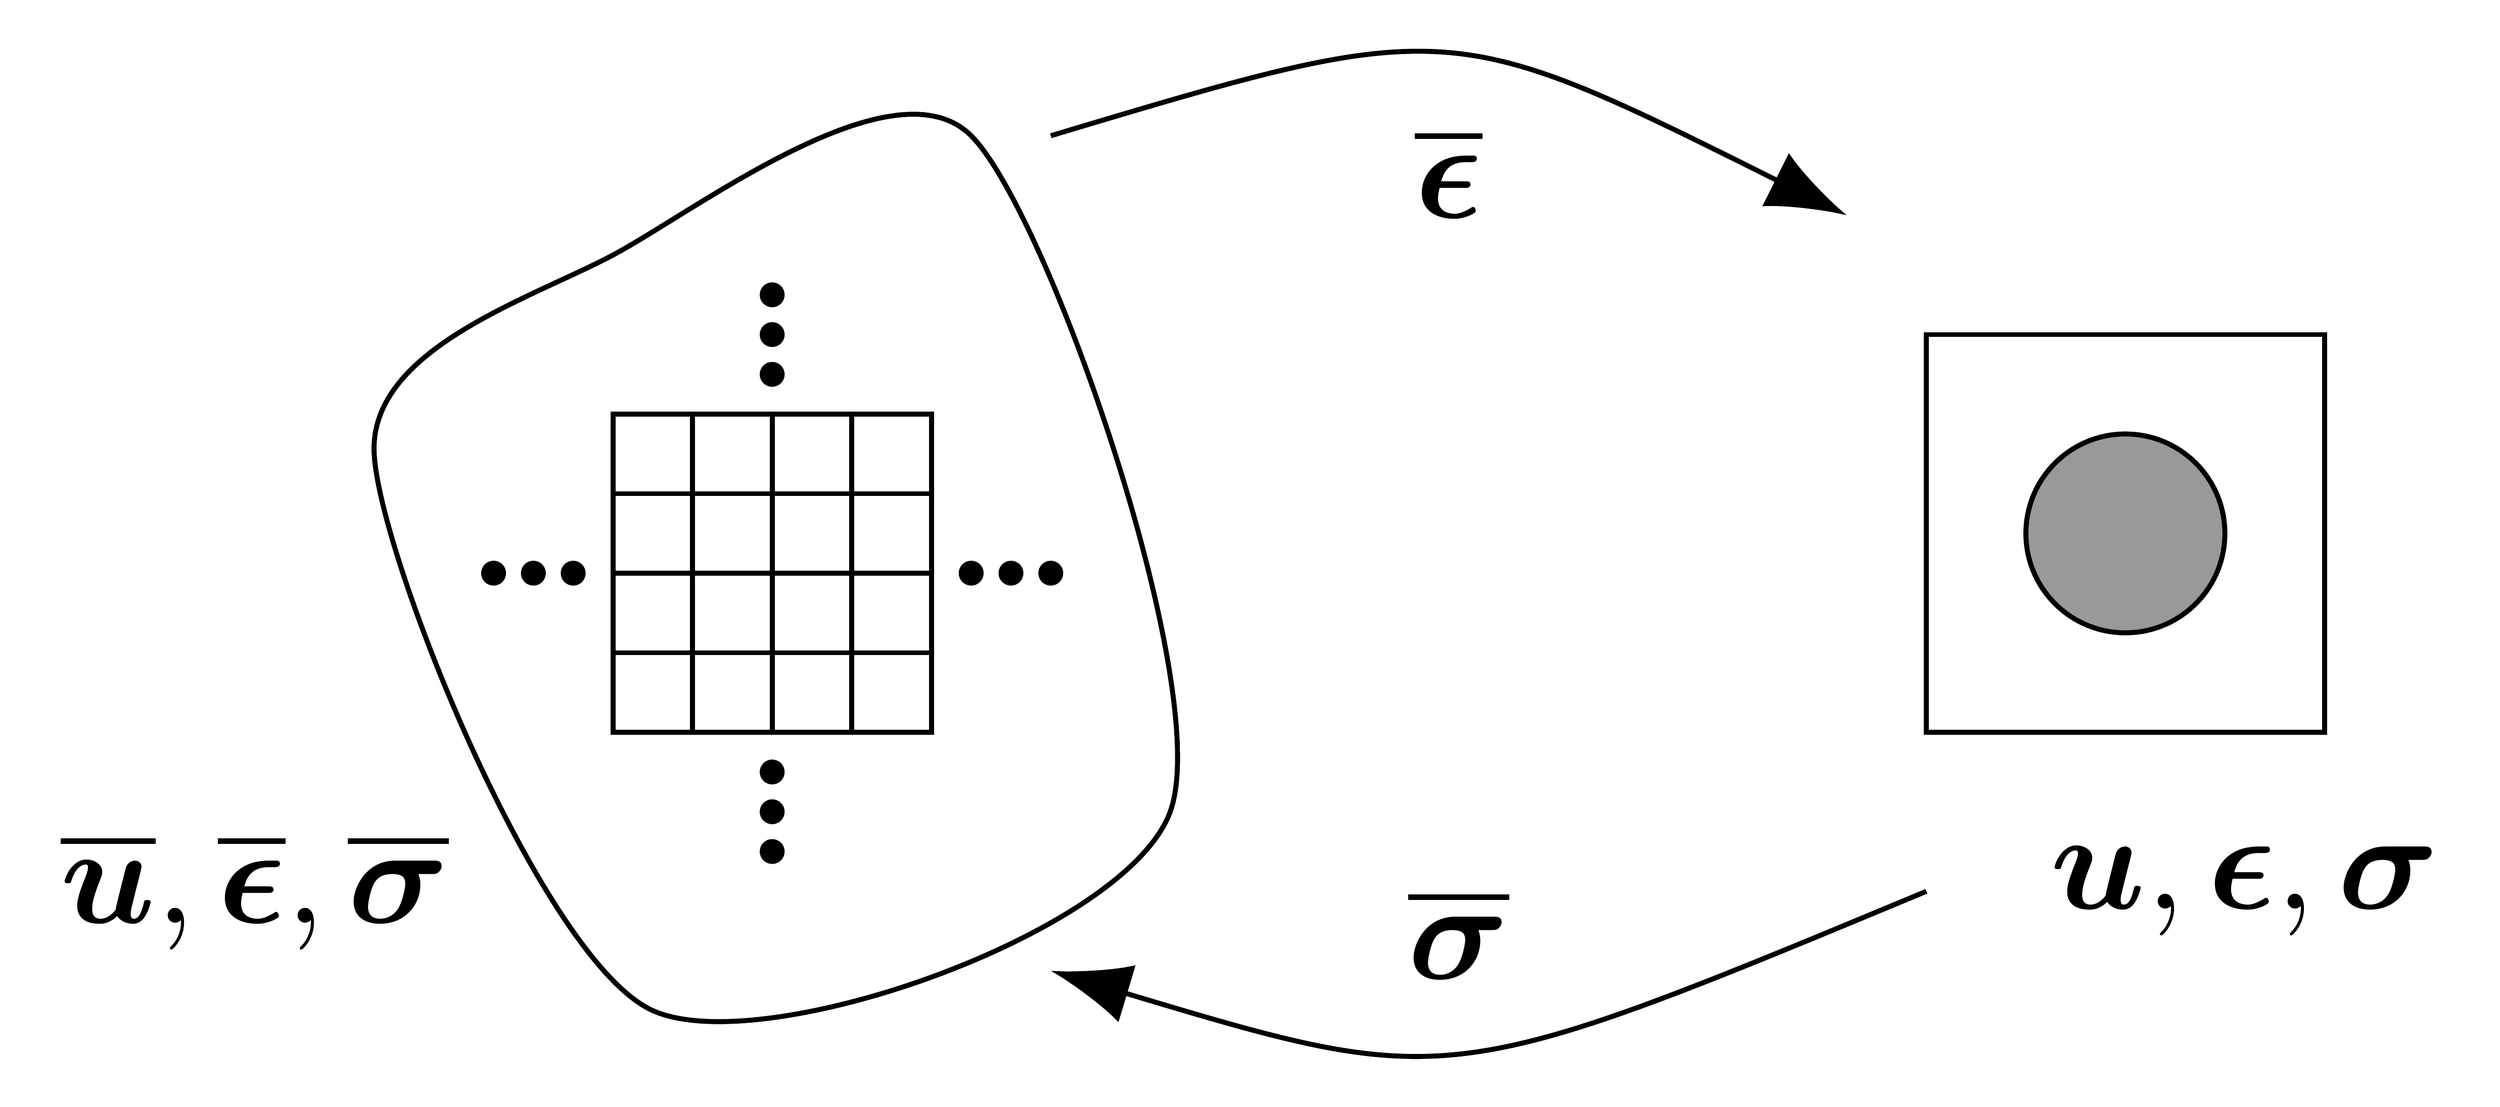
\begin{tikzpicture}[>=latex,node distance=0pt, line width=1.25mm]

% the h.m.s.

    %\draw [gray!50]  (2,0) -- (13,1) -- (26,6) -- (15,23) -- (1,20) -- cycle;
    \draw [black] plot [smooth cycle] coordinates {(6,15) (13,1) (26,6) (21,23)
    (12,20)};

    \begin{scope}[yshift = 0 cm,xshift = 4 cm]

    \foreach \y [count=\n]in {8,10,12,14}{ 
       \foreach \x [count=\n]in {8,10,12,14}{ 
         \begin{scope}[yshift = \y cm,xshift = \x cm,start chain=going right]
           \draw (0,0) -- (2,0) -- (2,2) -- (0,2) -- cycle;
           %\filldraw[fill=black!40!white,draw=black] (1,1) circle (0.5cm);
         \end{scope}
       }
    }

    \filldraw[fill=black,draw=black] (5,12) circle (0.25cm);
    \filldraw[fill=black,draw=black] (6,12) circle (0.25cm);
    \filldraw[fill=black,draw=black] (7,12) circle (0.25cm);

    \filldraw[fill=black,draw=black] (17,12) circle (0.25cm);
    \filldraw[fill=black,draw=black] (18,12) circle (0.25cm);
    \filldraw[fill=black,draw=black] (19,12) circle (0.25cm);

    \filldraw[fill=black,draw=black] (12,5) circle (0.25cm);
    \filldraw[fill=black,draw=black] (12,6) circle (0.25cm);
    \filldraw[fill=black,draw=black] (12,7) circle (0.25cm);

    \filldraw[fill=black,draw=black] (12,17) circle (0.25cm);
    \filldraw[fill=black,draw=black] (12,18) circle (0.25cm);
    \filldraw[fill=black,draw=black] (12,19) circle (0.25cm);

    \end{scope}

% the r.v.e.

    \begin{scope}[yshift = 8 cm,xshift = 45 cm,start chain=going right,scale=5]
          \draw (0,0) -- (2,0) -- (2,2) -- (0,2) -- cycle;
          \filldraw[fill=black!40!white,draw=black] (1,1) circle (0.5cm);
    \end{scope}

    \draw[-{Latex[length=20mm,width=15mm]}] (23,23) ..  controls ++(10,+3) ..
    node[below, scale=10] {$\overline{\bm{\epsilon}}$} 
    ++(20,-2);
    \draw[{Latex[length=20mm,width=15mm]}-] (23,2) .. controls ++(10,-3) .. 
    node[above, scale=10] {$\overline{\bm{\sigma}}$}
    ++(22,+2);

    \node[scale=10] at (3,4) {$\overline{\bm{u}}, \overline{\bm{\epsilon}}, \overline{\bm{\sigma}}$} ;
    \node[scale=10] at (53,4) {${\bm{u}}, {\bm{\epsilon}}, {\bm{\sigma}}$} ;


\end{tikzpicture}

\end{document}

}
\caption{\label{fig:multi-scale}Simplified scheme of a multi-scale calculation 
where at the left we have an homogenized macro-structure and 
in the right we have a representative volume element (\emph{r.v.e.}) 
representing the micro-structure.}
\end{figure}

We are going to develop first the equations that governs the macro scale
to arrive finally to a constitutive law that depends on a calculation over the
micro-scale.

The statical equilibrium for the macro-scale is governed by the equation

% <macro equilibrium equations>
\begin{equation}
\text{div } \overline{\bm{\sigma}} = \bm{0} \text{ in } \overline{V},\\
\label{eq:macro_equil}
\end{equation}

\noindent
where $\overline{\bm{\sigma}}$ represents the macroscopic stress and
$\overline{V}$ the volume of the whole structure. It is important to remark that
we have neglected the body and inertial forces terms because they do not
play a central role in our stiffness analysis.

% <epsilon = f(u)>
\begin{equation}
 \bm{\epsilon}_{ij} = \frac{1}{2}\left( \bm{u}_{i,j} + \bm{u}_{j,i} \right).
\label{eq:constitutive}
\end{equation}

While the strain $\bm{\sigma}$ in a linear elastic material can be defined with the 
constitutive relation :

% <constitutive relation>
\begin{equation}
\bm{\sigma}(\bm{u}) = \mathbb{C} : \bm{\epsilon}(\bm{u}).
\label{eq:constitutive}
\end{equation}

In the discretized version of the equations we want to avoid reaching 
the smallest heterogeneity scale, in practical examples this corresponds 
to the fibers' diameter. The main reason to avoid this is because, as we 
stated above, we would end in a huge computational cost problem.
The idea of the \emph{multi-scale} method is to calculate this value
as:

% <sigma average>
\begin{equation}
\overline{\bm{\sigma}} = \frac{1}{V} \int_{V} \bm{\sigma} dV,
\label{stress_ave}
\end{equation}

\noindent
where $V$ is the volume of a
representative volume element that takes into account all the details of the
heterogeneities of the micro-structure and $\bm{\sigma}$ is the microscopic
stress which is a representative field inside $V$ of what is happening in a
``small''\footnote{The size of the region in this case is not measure in
distance units but in distances relations between the macroscopic maximum length
$\overline{\ell}$ and the microscopic smallest length $\ell$.} region of the micro-structure.

% <epsilon average>
\begin{equation}
\overline{\bm{\varepsilon}} = \frac{1}{V} \int_{V} \bm{\varepsilon} dV,
\label{strain_ave}
\end{equation}

% <micro equations>
\begin{equation}
\left\{
\begin{array}{ll}
\text{div } \bm{\sigma} = 0 \\
\langle \bm{\epsilon} \rangle =  \overline{\bm{\epsilon}} \\
\bm{u} = \overline{\bm{\epsilon}} \cdot \bm{x}
\end{array}
\right.
\label{micro_eqs}
\end{equation}

\noindent
where \emph{b.c.} denotes the boundary conditions imposed. This boundary
conditions should be reproduce as close as possible the boundary conditions that
the  \emph{in-situ condition} that the cell has inside the structure. How this
cell is deformed is something that we do not know and we should assume. How well
we approximate this is how well the method will work.

It is easy to prove that imposing Dirichlet boundary conditions on all the
surface ($\partial V$) the value of $\langle \epsilon \rangle$ can be
immediately calculated. In this work we are going to explore the condition 
$ u = E \cdot y $ which gives $\langle \epsilon \rangle = E$ as we need. It
should be remark that different \emph{b.c.} can give the same result for example 
periodic \emph{b.c.} and uniform stress Neumann conditions work.

\subsection{Boundary conditions}

Three types of boundary conditions are often considered at the time \fe method is applied. 

\begin{itemize}
\item uniform strain
\item periodics
\item uniform stress
\end{itemize}

\subsubsection{Uniform strain}

\subsubsection{Periodic boundary conditions}

In this conditions we it is ask periodicity for the displacements field and anti-periodicity for the tension on the
surface.
First of all we have to define surfaces where we consider that the periodicity of this fields should happen.
For the two-dimensional square domain that we use in this work it seems reasonable to select the two pair of opposite parallel faces 
as we show on figure~\ref{fig_periodic_square}.
There, we select the points, except those in the corners, with a group nomenclature $\Gamma^+$ and $\Gamma^-$ that they
can be represented as:

\begin{equation}
\Gamma^+ = \{ \bm{x} = (x_1, x_2) \in \Gamma \,\setminus\, (x_1 = \ell_x \,\vee\, x_2 = \ell_y) \,\wedge\,
\bm{x}\neq(0,0) \,\wedge\,  \bm{x}\neq(\ell_x,0) \,\wedge\, \bm{x}\neq(0,\ell_y) \}
\end{equation}
\begin{equation}
\Gamma^- = \{ \bm{x} = (x_1, x_2) \in \Gamma \,\setminus\, (x_1 = 0 \,\vee\, x_2 = 0) \,\wedge\,
  \bm{x}\neq(\ell_x,0) \,\wedge\, \bm{x}\neq(\ell_x,\ell_y) \,\wedge\, \bm{x}\neq(0,\ell_y) \}
\end{equation}

Then for every point $\bm{x}^+ \in \Gamma^+$ we will assign a symmetric point $\bm{x}^- \in \Gamma^-$ that will we in
the nearest point on the opposite face of the square as we show in figure~\ref{fig_periodic_square}.

By this way the periodic condition for the displacement field on the surface will be state as:

\begin{equation}
\bm{u}^+ - \bm{u}^- = \overline{\bm{\epsilon}} (\bm{x}^+ - \bm{x}^-),
\end{equation}

\noindent
and the condition for the anti-periodic tractions will be:

\begin{equation}
\bm{\sigma}^{+} \cdot\hat{n}^+ + \bm{\sigma}^{-} \cdot\hat{n}^- = 0,
\end{equation}

\noindent
where $\bm{\sigma}^{+} = \bm{\sigma}(\bm{x}^{+})$ and $\bm{\sigma}^{-} = \bm{\sigma}(\bm{x}^{-})$
and $\hat{n}^+ = \hat{n}(\bm{x}^{+})$ and $\hat{n}^- = \hat{n}(\bm{x}^{-})$ the last are the unit normal vectors 
at those point respectively while the product $\bm{\sigma}\cdot\hat{n}$ represents the surface force at that point.

\subsubsection{Uniform stress}

In the next sections we are going to explain how can they be implemented using a FE discretization of the equations.

\subsection{Mixture theory}

Mixture theory was one of the first theories developed to explain the composite
material behavior and are relatively easy to apply. 
To explain briefly these theories we suppose linear constitutive relations for 
both materials of the composite, i.e.:

\begin{equation}
\Delta \bm{\sigma}_m = \mathbb{C}_m  \Delta \bm{\epsilon}_m 
\quad\text{and}\quad 
\Delta \bm{\sigma}_i = \mathbb{C}_i  \Delta \bm{\epsilon}_i,
\label{eq:const_im}
\end{equation}

\noindent
where $\mathbb{C}_m$, $\mathbb{C}_m$ are the constitutive tensor for the
\emph{matrix} and the \emph{fiber} materials respectively.

%-------------------------------------------------
\subsubsection{Parallel mixing theory}

Parallel mixture theory supposed both constitutive materials are align in parallel (in the
direction of the applied forces) and the
strains inside them is uniform and the same for both, i.e.:

\begin{equation}
\langle\Delta \bm{\epsilon}\rangle = \Delta \bm{\epsilon}_i = \Delta \bm{\epsilon}.
\end{equation}

\noindent
On the other hand, the total force can be calculated as a proportional
contribution of the forces applied by each part, i.e.:

\begin{equation}
\langle\Delta \bm{\sigma}\rangle  = v_m \Delta \bm{\sigma}_m + v_i \Delta \bm{\sigma}_i.
\end{equation}

Finally using the constitutive relations \ref{eq:const_im} we can arrive to the
approximation:

\begin{equation}
\mathbb{C}_p = \frac{\langle\Delta \sigma\rangle}{\langle\Delta \bm{\epsilon}\rangle} = 
v_m\frac{\Delta \bm{\sigma_m}}{\Delta \bm{\epsilon_m}} +
v_i\frac{\Delta \bm{\sigma_i}}{\Delta \bm{\epsilon_i}} = 
\mathbb{C}_m + \mathbb{C}_i
\label{eq:parallel_mix}
\end{equation}

%-------------------------------------------------

\subsubsection{Serial mixing theory}
In the serial theory we suppose constituent materials are in 
parallel (in the direction of the forces) so in
this case the forces in the materials are the same :

\begin{equation}
\langle \Delta \bm{\sigma} \rangle= \Delta \bm{\sigma}_i = \Delta \bm{\sigma},
\end{equation}

\noindent
and the total deformation is a proportional contribution of each part, i.e.:

\begin{equation}
\Delta \bm{\epsilon} = v_m \Delta \bm{\epsilon}_m + v_i \Delta \bm{\epsilon}_i
\end{equation}

Finally using Eq.~\ref{eq:const_im} we get

\begin{equation*}
\mathbb{C}_s^{-1} = \frac{\langle\Delta \epsilon\rangle}{\langle\Delta \sigma\rangle} = 
v_m\frac{\Delta \epsilon_m}{\Delta \sigma_m} +
v_i\frac{\Delta \epsilon_i}{\Delta \sigma_i} = 
\mathbb{C}_m^{-1} + \mathbb{C}_i^{-1}
\end{equation*}

\begin{equation}
\mathbb{C}_s =
\left( \mathbb{C}_m^{-1} + \mathbb{C}_i^{-1} \right)^{-1}
\label{eq:serial_mix}
\end{equation}

A more detailed reference about the parallel and serial mixture theory can be seen in the
reference~\cite{oller-composites} where the analysis is presented in an
energetic point of view.

%-------------------------------------------------

\subsection{Finite element discretization}

For solving numerically the \emph{multi-scale} problem we use the
FE-method in both scales.
In this work the \emph{micro} and \emph{macro}-problems 
are described by the same equilibrium equations so the discretization will
be the same for both. The notation that we will use here is the same used for
the \emph{micro}-problem.
To derive the discrete equations we start from the week form
of Eq.~\ref{eq:macro_equil} that can be state directly using the \emph{virtual work
principle}, a detail explanation of this can be found on reference~\cite{bathe-virt-work}.
The principle can be state in a variational sence as

% <principle of virtual work>
\begin{equation}
\int_V \bm{\sigma}(\bm{u}) : \delta \bm{\epsilon}(\bm{v})
\, dV = \bm{0} \quad \forall \quad \bm{v} \in \bm{\mathsf{V}}(V),
\end{equation}

\noindent
where $\delta \bm{\epsilon}$ are called \emph{virtual strains} and the vector
space $\bm{\mathsf{V}}(V)$ is defined as:

\begin{equation}
\bm{\mathsf{V}}(V) =
\{ 
  \bm{v} \in \left[\bm{\mathsf{H}}^1(V)\right]^2: \bm{v}=0 \text{ in } \partial V_d
\}.
\end{equation}

\noindent
notice that $\bm{v} \in \left[\bm{\mathsf{H}}^1(V)\right]^2$ means 
$\bm{v}_j \in \bm{\mathsf{H}}^1(V) \text{ for } j=1,2$ and $\bm{\mathsf{H}}^1(V) $ 
represents the Hilbert space

% <Hilbert space>
\begin{equation}
\bm{\mathsf{H}}^1(V) = \{ 
  v : v \in \bm{\mathsf{L}}_2(V): \frac{\partial v}{\partial x_i}=0 \in \bm{\mathsf{L}}_2(V)
  \text{ if } i=1,2 
\},
\end{equation}

\noindent
where $\bm{\mathsf{L}}_2(V)$ is the space of \emph{square integrable functions} in $V$
i.e.:
% <L2 space>
\begin{equation}
\bm{\mathsf{L}}_2(V) = \{ 
  v : v \text{ is defined in } V \text{ and } \int_V v^2 \, dV < \infty
\}.
\end{equation}

These definitions of vector spaces are the ones proposed by
Johnson~\cite{johnson-first} and allows to prove existence and uniqueness
solutions for the week form of this problem.

Before applying the FE discretization we should discretize the domain into finite
volumetric parts called elements, here we used triangles and quadrangles to mesh
the 2D domain $V$, $V \approx \cup_e V_e$ i.e. with one node in each vertex.
Then we construct a finite-dimensional space 
$\bm{\mathsf{V}}_h \subset \bm{\mathsf{V}}$, in this work we consider the
particular

\begin{equation}
\bm{\mathsf{V}}_h(V) = \{ 
  \bm{v} : \bm{v}_j \text{ continuos with piecewise partial derivatives in } V
  \text{ for } j=1,2
\}.
\end{equation}

A base for this space can be build taking the so called shape functions
$\varphi_i$ defined as 1 in node $i$, 0 in the rest of nodes and linear on
space. For finite elements operations we can defined the on \emph{master}
elements that are element that can be map to the real ones the conform the mesh.
In this work we use triangles and quadrangles in a 2D domain so these elements
are unity-like element as shown in
figures~\ref{fig:tria_master}~and~\ref{fig:quad_master} for the master triangle
and quadrangle respectively.

%-------------------------------------------------

% Master elements
\begin{figure}[!ht]
\centering
\begin{minipage}[b]{0.4\linewidth}
\subcaptionbox{\label{fig:tria_master}}{
\resizebox{4.0cm}{!}{\documentclass{standalone}
\begin{document}
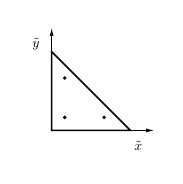
\begin{tikzpicture}[>=latex,node distance=0pt, line width=0.2mm]

 \draw []  (0,0) -- (1,0) -- (0,1) -- cycle;
 \draw [-{Latex[length=1.0mm,width=0.5mm]}, line width=0.1mm]  (1,0) -- (1.3,0) ;
 \draw [-{Latex[length=1.0mm,width=0.5mm]}, line width=0.1mm]  (0,1) -- (0,1.3) ;

 \draw[fill=black](.166,0.166) circle (0.1mm);
 \draw[fill=black](.666,0.166) circle (0.1mm);
 \draw[fill=black](.166,0.666) circle (0.1mm);
 
 \node[scale=0.5] at (+1.1,-0.2) {$\tilde{x}$};
 \node[scale=0.5] at (-0.2,+1.1) {$\tilde{y}$};
 
 % define a cross X
 \tikzset{cross/.pic={
  \draw []  (0,0) -- (1,1) ;
  \draw []  (1,0) -- (0,1) ;
 }}
 %\draw []  (0.166,0.166) pic[scale=0.03] {cross};
 %\draw []  (0.666,0.166) pic[scale=0.03] {cross};
 %\draw []  (0.166,0.666) pic[scale=0.03] {cross};

\end{tikzpicture}
\end{document}

}}
\end{minipage}
\hspace{1.5cm}
\begin{minipage}[b]{0.4\linewidth}
\subcaptionbox{\label{fig:quad_master}}{
\resizebox{4.0cm}{!}{\documentclass{standalone}
\begin{document}
\begin{tikzpicture}[>=latex,node distance=0pt, line width=0.2mm]

 \draw []  (0,0) -- (1,0) -- (1,1) -- (0,1)-- cycle;
 \draw [-{Latex[length=1.0mm,width=0.5mm]}, line width=0.1mm]  (0,0) -- (1.3,0) ;
 \draw [-{Latex[length=1.0mm,width=0.5mm]}, line width=0.1mm]  (0,0) -- (0,1.3) ;

 \draw[fill=black](0.211,0.211) circle (0.1mm);
 \draw[fill=black](0.788,0.211) circle (0.1mm);
 \draw[fill=black](0.788,0.788) circle (0.1mm);
 \draw[fill=black](0.211,0.788) circle (0.1mm);
 
 \node[scale=0.5] at (+1.1,-0.2) {$\tilde{x}$};
 \node[scale=0.5] at (-0.2,+1.1) {$\tilde{y}$};
 
 % define a cross X
 \tikzset{cross/.pic={
  \draw []  (0,0) -- (1,1) ;
  \draw []  (1,0) -- (0,1) ;
 }}
 %\draw []  (0.166,0.166) pic[scale=0.03] {cross};
 %\draw []  (0.666,0.166) pic[scale=0.03] {cross};
 %\draw []  (0.166,0.666) pic[scale=0.03] {cross};

\end{tikzpicture}
\end{document}
}}
\end{minipage}
\caption{Master element to perform the FEM integrals.
a) Master triangle element. 
b) Master quadrangle element.
}
\label{fig_dist_scheme}
\end{figure}

%-------------------------------------------------

Then the master shape functions for the space $\bm{\mathsf{V}}_h$ are defined as

% <master shape functions>
\begin{equation}
\left\{
\begin{array}{ll}
\tilde{\varphi}_1(\tilde{x},\tilde{y}) = 1 - \tilde{x} - \tilde{y}\\
\tilde{\varphi}_2(\tilde{x},\tilde{y}) = \tilde{x}\\
\tilde{\varphi}_3(\tilde{x},\tilde{y}) = \tilde{y}\\
\end{array}
\right.
\quad
\left\{
\begin{array}{ll}
\tilde{\varphi}_1(\tilde{x},\tilde{y}) = (1 - \tilde{x})(1 - \tilde{y})\\
\tilde{\varphi}_2(\tilde{x},\tilde{y}) = \tilde{x}(1 - \tilde{y})\\
\tilde{\varphi}_3(\tilde{x},\tilde{y}) = \tilde{x}\tilde{y}\\
\tilde{\varphi}_4(\tilde{x},\tilde{y}) = (1 - \tilde{x})\tilde{y}\\
\end{array}
\right.
.
\end{equation}

Then every integral on the elements containing shape functions and it derivatives as arguments
can be calculated simply by

% < phi x phi>
\begin{equation}
\int_{V_{e}} \varphi_i \varphi_j dV = \sum_{g}
\tilde{\phi_i}(\tilde{x}_g,\tilde{y}_g) 
\tilde{\phi_j}(\tilde{x}_g,\tilde{y}_g) 
w_g |\bm{J}_g|
\end{equation}

% < d_phi x d_phi>
\begin{equation}
\int_{V_{e}} \partial_{x_i}\varphi_i \partial_{x_j}\varphi_j dV = \sum_{g}
\left[
\bm{J}_g^{-1}\partial_{\tilde{x}_i}\tilde{\phi_i}(\tilde{x}_g,\tilde{y}_g)
\right]
\left[
\bm{J}_g^{-1}\partial_{\tilde{x}_i}\tilde{\phi_j}(\tilde{x}_g,\tilde{y}_g) 
\right]
w_g |\bm{J}_g|
\end{equation}

where we use the Gaussian quadrature of points $(\tilde{x}_g,\tilde{y}_g)$
summarised on table~\ref{tab:gauss}. On the other hand $\bm{J}$ is the
Jacobian matrix of the linear coordinate transformation inside an elements of
$N_v$ verteces with coordinates $\bm{x_i}$

% < x = sum phi(x_m) >
\begin{equation}
\bm{x} =
\sum_{i}^{N_{v}} \bm{x}_i \tilde{\varphi}_i (\tilde{\bm{x}})
\end{equation}

Then
% < x = sum phi(x_m) >
\begin{equation}
\partial_{\tilde{x}_i} \varphi =
\partial_{x_i} \varphi
\partial_{\tilde{x}_i} \bm{x} 
\Rightarrow 
\nabla_{\tilde{\bm{x}}} \varphi =
\bm{J}
\nabla_{\bm{x}} \varphi \text{ with }
\bm{J}_{ij} = 
\partial_{\tilde{x}_j} x_i 
\end{equation}


%-------------------------------------------------

% < Gauss point table >
\begin{table}[ht]
\centering
\begin{tabular}{ | c | c | c | }
\hline
& triangle & quadrangle \\ 
\hline
1 &($\frac{1}{6}$,$\frac{1}{6}$)& ($\frac{\sqrt{3}-1}{2\sqrt{3}}$,$\frac{\sqrt{3}-1}{2\sqrt{3}}$)\\
2 &($\frac{2}{3}$,$\frac{1}{6}$)& ($\frac{\sqrt{3}+1}{2\sqrt{3}}$,$\frac{\sqrt{3}-1}{2\sqrt{3}}$)\\
3 &($\frac{1}{6}$,$\frac{2}{3}$)& ($\frac{\sqrt{3}+1}{2\sqrt{3}}$,$\frac{\sqrt{3}+1}{2\sqrt{3}}$)\\
4 &                             & ($\frac{\sqrt{3}-1}{2\sqrt{3}}$,$\frac{\sqrt{3}+1}{2\sqrt{3}}$)\\
\hline 
\end{tabular}
\caption{\label{tab:gauss}}
\end{table}

%-------------------------------------------------

The discretized weak form can be state now as
% <weak form>
\begin{equation}
\int_V \delta \bm{\epsilon}(\bm{v}_h) : \mathbb{C} : \bm{\epsilon}(\bm{v}_h) \,dV = \bm{0}
\quad \forall \quad \bm{v}_h \in \bm{\mathsf{V}}_h(V),
\end{equation}

\noindent
taking $\bm{v}_h = \psi_i$, i.e. the elements of the base, we
arrive to a system of linear equations.

\begin{equation}
\overline{\bm{u}}^i(\bm{x}) = 
\sum_{j=1}^N \bm{u}_j^i \varphi_j (\bm{x})
\end{equation}

\begin{equation}
\int_V \delta \bm{\epsilon}:\bm{\sigma} \,dV
\approx
\sum_i \int_{V_i} \delta \bm{\epsilon}:\bm{\sigma} \,dV
\end{equation}

\begin{equation}
\bm{K}\bm{U} = \bm{b}
\label{eq:equil_matricial}
\end{equation}

%-------------------------------------------------

\subsection{Modal analysis}

The objective of the modal analysis is to calculate the natural frequencies
of a system, these are important in the design of the structures because we can avoid 
high amplitude oscillations and, as a consequence, the failure of the material. 
For calculating the natural frequencies of the system we should start from the
dynamic equation  

% <macro motion equations>
\begin{equation}
\rho \ddot{\bm{u}} + \text{div } \bm{\sigma} = \bm{0} \text{ in } V,
\label{eq:motion}
\end{equation}

\noindent
in which we have neglected the dissipative terms and external body and surface
forces.
Assuming that the solution $\overline{\bm{u}}$ can be expressed as the
product of a function that depends only on time $f(t)$ and a function that
depend only on space $\bm{g}(\overline{\bm{x}})$ 

% <variables' separation>
\begin{equation}
\bm{u}(t,\overline{\bm{x}}) = f(t) \bm{g}(\bm{x}),
\label{eq:u_fg}
\end{equation}

\noindent
and considering that the stress $\bm{\sigma}$ only depends on the
spatial derivatives of $\bm{u}$ we can write:

% <macro motion equations>
\begin{equation}
\rho \ddot{f}(t) \bm{g}(\bm{x}) +
f(t) \text{div } \overline{\bm{\sigma}}(\bm{g}(\bm{x}))
= \bm{0} \text{ in } V.
\label{eq:motion_subs_fg}
\end{equation}

We can solve the time part of this equation with solutions of the form

% < f = sin >
\begin{equation}
f_i(t) = \sin (\omega_i t + \varphi).
\label{eq:f_sin}
\end{equation}

\noindent
and an associated function $\bm{g}_i$. The idea is that if we substitute 
on Eq.~\ref{eq:motion_subs_fg} we get

\begin{equation}
- \rho \omega_i^2 \sin (\omega_i t + \varphi) \bm{g}_i(\bm{x}) +
\sin (\omega_i t + \varphi) \text{div } \bm{\sigma}(\bm{g}_i(\bm{x})) 
= \bm{0} \text{ in } V,
\label{eq:motion}
\end{equation}

\noindent
the term $\sin (\omega_i t + \varphi)$ vanish and gives

\begin{equation}
- \rho \omega_i^2 \bm{g}_i(\bm{x}) +
\text{div } \bm{\sigma}(\bm{g}_i(\bm{x})) 
= \bm{0} \text{ in } V.
\label{eq:motion}
\end{equation}

This mean that any solution of Eq.~\ref{eq:motion} can be expressed as a linear
combination of functions like \ref{eq:f_sin} because of the \emph{Dirichlet
theorem}:

\begin{equation}
\bm{u}(t,\bm{x}) = \sum_{i=1}^{\infty} f_i(t)
\bm{g}_i(\bm{x}).
\label{eq:dir_teo}
\end{equation}

The equation can be written in a more convenient way

\begin{equation}
\rho \bm{g}_i(\bm{x}) = 
\lambda_i  \text{ div } \bm{\sigma}(\bm{g}_i(\bm{x})) 
\text{ in } V,\\
\label{eq:motion}
\end{equation}

\noindent
where the functions $\bm{g}_i(\overline{\bm{x}})$ are called eigenvectors and the
values $\lambda_i$ are called eigenvalues and are directly related with the
natural frequencies by the formula

\begin{equation}
\lambda_i = \frac{1}{\omega_i^2}.
\label{eq:motion}
\end{equation}

\begin{equation}
\bm{M}\bm{U} = \lambda \bm{K}\bm{U}
\label{eq:equil_matricial}
\end{equation}

%---------------------------------------------------------------------------------------------------

\section{Numerical Implementation of the Micro-problem}

\subsection{Uniform Strains Boundary Conditions}

\subsection{Periodic Boundary Conditions}

\begin{equation}
\left\{
\begin{array}{ll}
\bm{f}_a(\bm{u}) = \bm{0} \\
\bm{f}_b^+(\bm{u}) + \bm{f}_b^-(\bm{u}) = \bm{0} \\
\bm{u}^+ - \bm{u}^- - \overline{\bm{\epsilon}} ( \bm{x}^+ - \bm{x}^- ) = \bm{0}\\
\end{array}
\right.
\end{equation}

\begin{equation}
\bm{c}(\bm{x}) = \overline{\bm{\epsilon}} ( \bm{x}^+ - \bm{x}^- ) \\
\end{equation}

\begin{equation}
\bm{u}^+ - \bm{u}^- - \bm{c}(\bm{x}) = \bm{0}
\end{equation}

\subsubsection{The Unknowns Elimination Method}

\begin{equation}
\bm{u}^+ = \bm{u}^- + \bm{c}(\bm{x}) 
\end{equation}

\begin{equation}
\bm{u} = \begin{bmatrix}\bm{u}_a & \bm{u}_+ & \bm{u}_-\end{bmatrix}^T
\end{equation}

\begin{equation}
d\bm{u}^+ = d\bm{u}^-
\end{equation}

\begin{equation}
d\bm{u} = \begin{bmatrix}d\bm{u}_a & d\bm{u}_+ & d\bm{u}_-\end{bmatrix}^T = \begin{bmatrix}d\bm{u}_a & d\bm{u}_- & d\bm{u}_-\end{bmatrix}^T
\end{equation}

\begin{equation}
\begin{bmatrix}
\frac{\bm{f}_a}{d\bm{u}_a} & \frac{\bm{f}_a}{d\bm{u}_+} & \frac{\bm{f}_a}{d\bm{u}_-}\\
\frac{\bm{f}_b^+ + \bm{f}_b^-}{d\bm{u}_a} & \frac{\bm{f}_b^+ + \bm{f}_b^-}{d\bm{u}_+} & \frac{\bm{f}_b^+ + \bm{f}_b^-}{d\bm{u}_-}\\
\end{bmatrix}
\cdot
\begin{bmatrix}d\bm{u}_a \\ d\bm{u}_- \\ d\bm{u}_-\end{bmatrix}
=
\begin{bmatrix}
\bm{f}_a(\bm{u}) \\
\bm{f}_b^+(\bm{u}) + \bm{f}_b^-(\bm{u})
\end{bmatrix}^{k-1}
\end{equation}

\begin{equation}
\begin{bmatrix}
K_{aa}          & K_{a+} + K_{a-} \\
K_{+a} + K_{-a} & K_{++} + K_{-+}  + K_{+-} + K_{--} \\
\end{bmatrix}
\cdot
\begin{bmatrix}d\bm{u}_a \\ d\bm{u}_- \end{bmatrix}
=
-\begin{bmatrix}\bm{f}_a(\bm{u}^{k-1}) \\ \bm{f}_b^+(\bm{u}^{k-1}) + \bm{f}_b^-(\bm{u}^{k-1}) \end{bmatrix}
\end{equation}


The algorithm:

\begin{equation}
\bm{u}^{i=0} = \begin{bmatrix}\bm{u}_a^{0} \\ \bm{u}_+^{0} \\ \bm{u}_-^{0}\end{bmatrix} = \begin{bmatrix}\bm{0} \\ \bm{c} \\ \bm{0}\end{bmatrix}
\end{equation}

\begin{equation}
\bm{u}_a^{0} = \bm{0}, \, \bm{u}_-^{0} = 0 \text{ and } \bm{u}_+^{0} = \bm{u}_-^{0} + \bm{c} = \bm{c}
\end{equation}

\begin{equation}
\bm{J}^{i-1}\cdot d\bm{u}^{i}
=
-r(\bm{u}^{i-1})
\end{equation}


\begin{equation}
\bm{u}^{i+1} = 
\begin{bmatrix}\bm{u}_a^{i-1} \\ \bm{u}_+^{i-1} \\ \bm{u}_-^{i-1}\end{bmatrix} 
+ 
\begin{bmatrix} d\bm{u}_a^{i} \\ d\bm{u}_+^{i} \\ d\bm{u}_-^{i}\end{bmatrix}
\end{equation}

\subsubsection{The Lagrange Multipliers Method}

\begin{equation}
\left\{
\begin{array}{ll}
\bm{f}_a(\bm{u}) = \bm{0} \\
\bm{f}_b^+(\bm{u}) + \bm{\lambda} = \bm{0} \\
\bm{f}_b^-(\bm{u}) - \bm{\lambda} = \bm{0} \\
\bm{u}^+ - \bm{u}^- - \bm{c} = \bm{0}\\
\end{array}
\right.
\end{equation}

\begin{equation}
\begin{bmatrix}
\frac{\partial\bm{f}_a}{\partial\bm{u}_a} & \frac{\partial\bm{f}_a}{\partial\bm{u}_+} & \frac{\partial\bm{f}_a}{\partial\bm{u}_-} &  \bm{0}\\
\frac{\partial\bm{f}_+}{\partial\bm{u}_a} & \frac{\partial\bm{f}_+}{\partial\bm{u}_+} & \frac{\partial\bm{f}_+}{\partial\bm{u}_-} &  \mathbbm{1}\\
\frac{\partial\bm{f}_-}{\partial\bm{u}_a} & \frac{\partial\bm{f}_-}{\partial\bm{u}_+} & \frac{\partial\bm{f}_-}{\partial\bm{u}_-} & -\mathbbm{1}\\
\bm{0}                                    & \mathbbm{1}                               & -\mathbbm{1}                              &  \bm{0}\\
\end{bmatrix}^{k-1}
\cdot
\begin{bmatrix}
d\bm{u}_a \\
d\bm{u}_+ \\
d\bm{u}_- \\
d\bm{\lambda}
\end{bmatrix}^{k}
=
\begin{bmatrix}
\bm{f}_a(\bm{u}) \\
\bm{f}_b^+(\bm{u}) + \bm{\lambda} \\
\bm{f}_b^-(\bm{u}) - \bm{\lambda} \\
\bm{u}^{+} - \bm{u}^{-} - \bm{c}
\end{bmatrix}^{k-1}
\end{equation}

\begin{equation}
\begin{bmatrix}
\bm{u}_a \\
\bm{u}_+ \\
\bm{u}_- \\
\bm{\lambda}
\end{bmatrix}^{k}
= 
\begin{bmatrix}
\bm{u}_a \\
\bm{u}_+ \\
\bm{u}_- \\
\bm{\lambda}
\end{bmatrix}^{k-1}
+
\begin{bmatrix}
d\bm{u}_a \\
d\bm{u}_+ \\
d\bm{u}_- \\
d\bm{\lambda}
\end{bmatrix}^{k-1}
\end{equation}

\subsection{Uniform Stresses Boundary Conditions}

%---------------------------------------------------------------------------------------------------

\section{Numerical Examples}

In this section we analyze two bi-dimensional examples where we compare the accuracy of
the \emph{uniform strains}, \emph{parallel mixture} and \emph{serial mixture}
homogenization theories with the micro-model. The micro-model is enough small in
both cases to be solve computationally and we consider this model the
\emph{exact} solution of the problem:

$$\text{\emph{exact}} \equiv \text{\emph{micro-model}}.$$

For modeling the matrix and the fibers on the micro-structure we assume plane
state of strain. For this case the constitutive tensor in Voigt notation is 
(Ref.~\cite{chavez_continuo})

\begin{equation}
\mathbb{C} = 
\frac{E}{(1+\nu)(1-2\nu)}
  \begin{bmatrix}
  1-\nu    & \nu      & 0                  \\
  \nu      & 1-\nu    & 0                  \\
  0        & 0        & \frac{1}{2}(1-2\nu)\\
  \end{bmatrix},
\end{equation}

\noindent
where $E$ is the Young modulus and $\nu$ is the Poisson ratio.

We are going to differentiate these values from the matrix and fiber with $E_m$,
$\nu_m$, $E_i$ and $\nu_i$ respectively. In all the cases that we present the
values of this quantities are those express on Table~\ref{tab:e_nu}.

\begin{table}[ht]
\centering
%\resizebox{1.0\columnwidth}{!}
\caption{\label{tab:e_nu}Values of Young modulus ($E_m$ and $E_i$) and Poisson
Ratio ($\nu_m$ and $\nu_i$) for the matrix and the fiber respectively.}
\end{table}

These values remains the same in all the simulation except on the \emph{modal
analysis} calculations where we do a parametric analysis of the eigenvalues as a
function of $E_m$.

%---------------------------------------------------------------------------------------------------

\subsection{Frontal fibers}

In this example we simulate a square structure with 10$\times$10 circular fibers 
like the one shown on Fig.~\ref{fig:geo1_geom}. 
Two different meshes where used, one to simulate the problem with the
\emph{micro-model}: 
this consists on the one shown on Fig.~\ref{fig:geo1_mesh} with the squares
replaced by the \emph{rve} mesh shown at the top right.
And the one used to solve the problem with the homogenization theories:
which is the one shown on Fig.~\ref{fig:geo1_mesh} only with the blank 
10$\times$10 squares.


\begin{figure}[!ht]
\begin{minipage}[b]{0.47\linewidth}
\subcaptionbox{\label{fig:geo1_geom}}{
\resizebox{8.0cm}{!}{\documentclass{standalone}

\begin{document}

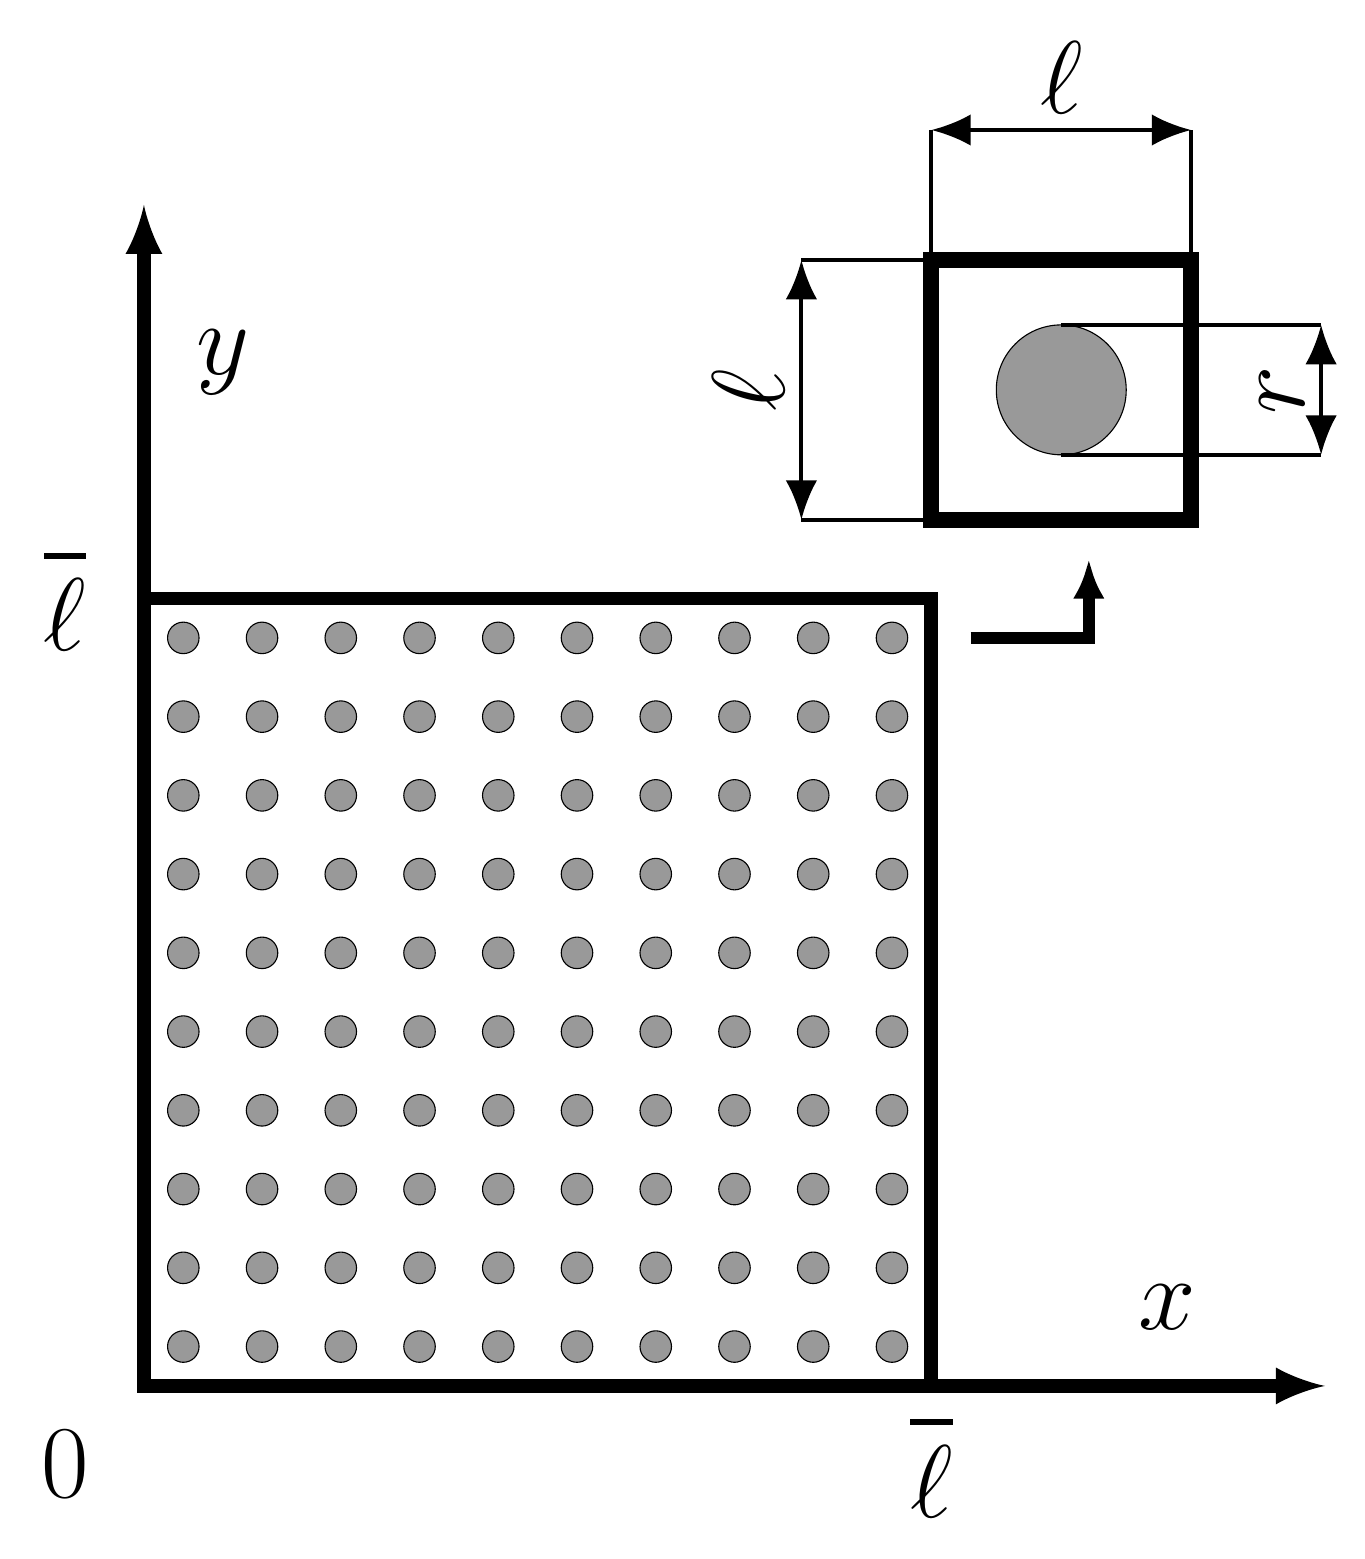
\begin{tikzpicture}[>=latex,node distance=0pt,font={\fontsize{40pt}{12}\selectfont}]

% structure
\foreach \y [count=\n]in {1,2,3,4,5,6,7,8,9,10}
{ 
  \foreach \x [count=\n]in {1,2,3,4,5,6,7,8,9,10}
  { 
    \begin{scope}[yshift = \y cm,xshift = \x cm,start chain=going right]
      %\draw (0,0) -- (4,0) -- (4,4) -- (0,4) -- cycle;
      \filldraw[fill=black!40!white,draw=black] (-0.5,-0.5) circle (0.20cm);
    \end{scope}
  }
}
\draw[line width=1.75mm] (0,0) -- (10,0) -- (10,10) -- (0,10) -- cycle;

\draw[-{Latex[length=5mm,width=4mm]}, line width=1.5mm] (10.5,9.5) -- ++(1.5,0)
  -- ++(0,1);

% rve
\begin{scope}[xshift=10.0cm,yshift=11cm, rotate=0.0, scale=1.1]

 \draw[draw=black, line width=2.0mm] (0,0) rectangle (3,3);
 \filldraw[fill=black!40!white,draw=black] (1.5,1.5) circle (0.75cm);
 
 \draw[line width=0.5mm] (1.5,2.25) -- ++(3,0);
 \draw[line width=0.5mm] (1.5,0.75) -- ++(3,0);
 \draw[{Latex[length=5mm,width=4mm]}-{Latex[length=5mm,width=4mm]},line width=0.5mm] 
 (4.5,0.75) --  node[above,rotate=90,scale=1.5] {$r$}  ++(0,1.5);

 \draw[line width=0.5mm] (0,3) -- ++(0,1.5);
 \draw[line width=0.5mm] (3,3) -- ++(0,1.5);
 \draw[{Latex[length=5mm,width=4mm]}-{Latex[length=5mm,width=4mm]},line width=0.5mm] 
 (0,4.5) --  node[above,scale=1.5] {$\ell$}  ++(3,0);
 
 
 
 \draw[line width=0.5mm] (0,3) -- ++(-1.5,0);
 \draw[line width=0.5mm] (0,0) -- ++(-1.5,0);
 \draw[{Latex[length=5mm,width=4mm]}-{Latex[length=5mm,width=4mm]},line width=0.5mm] 
 (-1.5,0.0) --  node[above,rotate=90,scale=1.5] {$\ell$}  ++(0,3);

\end{scope}

% axes
\draw[-latex,line width=1.75mm] (0,10) -- ++ (0, 5) ;
\draw[-latex,line width=1.75mm] (10,0) -- ++ (5, 0) ;
\node[scale=1.5] (a) at (13,1)  {$x$};
\node[scale=1.5] (a) at (1,13)  {$y$};
\node[scale=1.5] (a) at (-1,-1) {$0$};
\node[scale=1.5] (a) at (10,-1) {$\overline{\ell}$};
\node[scale=1.5] (a) at (-1,10) {$\overline{\ell}$};

\end{tikzpicture}

\end{document}
}}
\end{minipage}
\hspace{2.2cm}
\begin{minipage}[b]{0.47\linewidth}
\subcaptionbox{\label{fig:geo1_mesh}}{
\resizebox{8.0cm}{!}{\documentclass{standalone}

\begin{document}

\begin{tikzpicture}[>=latex,node distance=0pt,font={\fontsize{40pt}{12}\selectfont}]

    \draw[step=1cm,black] (0,0) grid (10,10);
    \node[inner sep=0pt, scale=0.5] (rve) at (12,12.5)
        {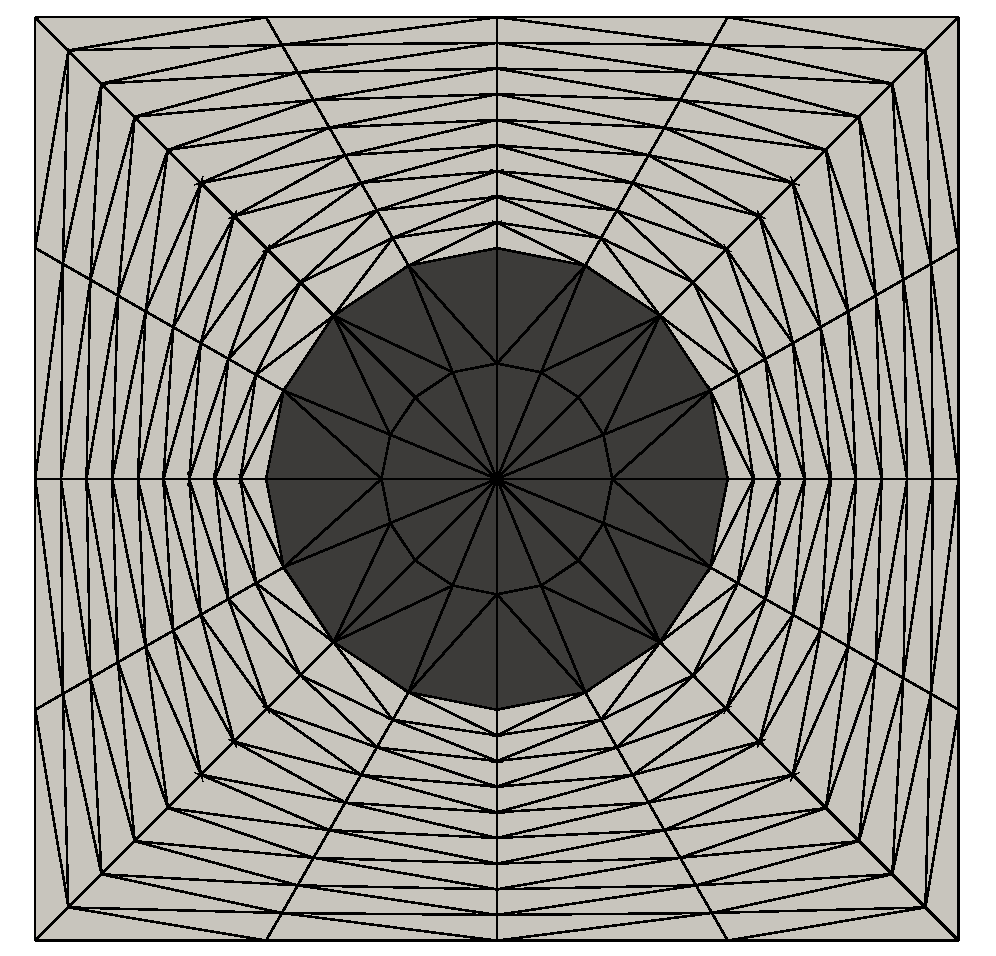
\includegraphics[width=1.4\textwidth]{figures/direct_mesh_frontal_zoom-crop.pdf}};
    \draw[draw=black, line width=2.0mm] (9,9) rectangle (10,10);
    \draw[-{Latex[length=5mm,width=4mm]}, line width=1.5mm] (10.5,9.5) -- ++(1.5,0)
    -- ++(0,1);

    % axes
    \draw[-latex,line width=1.75mm] (0,0) -- ++ (0, 15) ;
    \draw[-latex,line width=1.75mm] (0,0) -- ++ (15, 0) ;
    \node[scale=1.5] (a) at (13,1) {$x$};
    \node[scale=1.5] (a) at (1,13) {$y$};
    \node[scale=1.5] (a) at (-1,-1) {$0$};
    \node[scale=1.5] (a) at (10,-1) {$\overline{\ell}$};
    \node[scale=1.5] (a) at (-1,10) {$\overline{\ell}$};

\end{tikzpicture}

\end{document}

}}
\end{minipage}
\caption{Frontal fiber example. On \ref{fig:geo1_geom}) the problem description
         with zero displacement boundary condition and zero stress on the other faces. On
         \ref{fig:geo1_mesh}) the mesh used to solve the micro-model problem (with the
         substitution of the small \emph{rve} cell on the squares. The mesh with the
         squares with $n=20$ was used to solve the problem with the homogenization
         theories that are treat here. }
\label{fig_dist_scheme}
\end{figure}

\subsubsection{Homogenization model}

For all the homogenization models we use the structured grid code \micro that belongs to the 
free software \sputnik project ( Ref.~\cite{sputnik} ).
that is optimized for solve non-linear problems.

\begin{figure}[!ht]
\centering
\resizebox{5.0cm}{!}{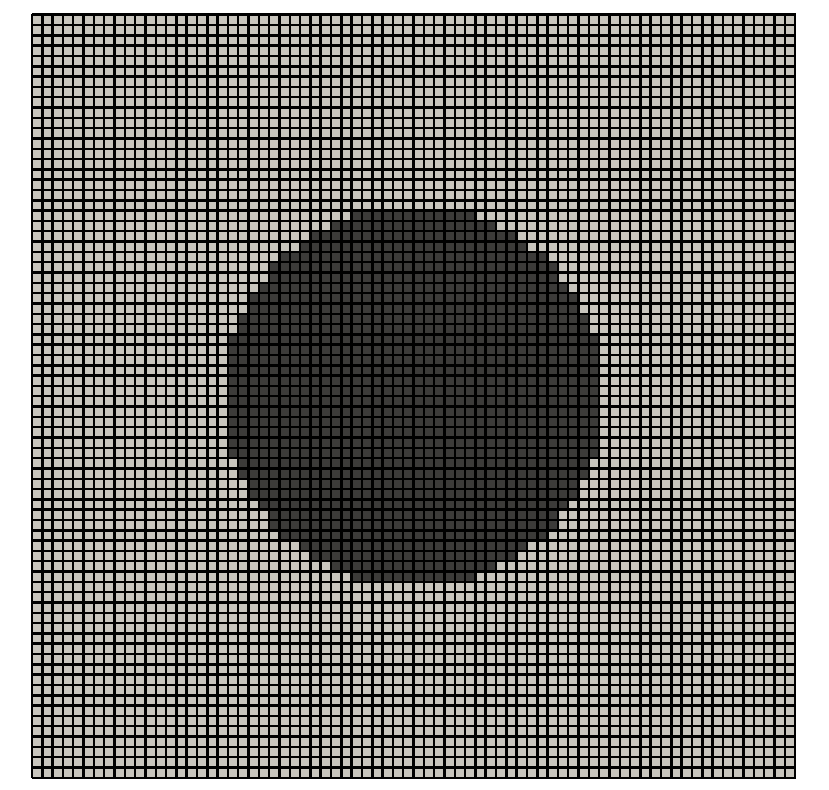
\includegraphics[width=1.4\textwidth]{figures/rve_5_msh-crop.pdf}}
\caption{Representative volume element to perform the homogenization calculation for obtaining the 
average properties $\overline{\bm{\sigma}}$ and $\overline{\mathbb{C}}$.}
\label{fig_rve_front_fib}
\end{figure}

\begin{equation}
\overline{\mathbb{C}}_h = 
  \begin{bmatrix}
   \begin{tabular}{ @{}*{3}{S[round-mode=places,
                    round-integer-to-decimal,round-precision=2,
                    table-format=1.2e4,table-column-width=16mm,table-number-alignment=center]}@{}
		  }
    1.7722e+06 & 7.08e+05 & 0.0\\
    7.08e+05 & 1.77e+06 & 0.0\\
    0.0          & 0.0  & 5.18e+05
   \end{tabular}
  \end{bmatrix}
\end{equation}

\begin{equation}
\overline{\mathbb{C}}_p = 
  \begin{bmatrix}
   \begin{tabular}{ @{}*{3}{S[round-mode=places,
                    round-integer-to-decimal,round-precision=2,
                    table-format=1.2e4,table-column-width=16mm,table-number-alignment=center]}@{}
		  }
    3.691352e+06 & 1.582008e+06 & 0.0\\
    1.582008e+06 & 3.691352e+06 & 0.0\\
    0.0          & 0.0          & 1.054672e+06
   \end{tabular}
  \end{bmatrix}
\end{equation}

\begin{equation}
  \overline{\mathbb{C}}_s = 
  \begin{bmatrix}
   \begin{tabular}{ @{}*{3}{S[round-mode=places,
                    round-integer-to-decimal,round-precision=2,
                    table-format=1.2e4,table-column-width=16mm,table-number-alignment=center]}@{}
		  }
    1.630150e+06 & 6.986357e+05 & 0.0\\
    6.986357e+05 & 1.630150e+06 & 0.0\\
    0.0          & 0.0          & 4.657572e+05
   \end{tabular}
  \end{bmatrix}
\end{equation}

We study two boundary condition cases for the micro structure

\begin{equation}
\left\{
\begin{array}{ll}
\overline{\bm{u}} = (0,0) \text{ in } x=0\\
\overline{\bm{u}} = \overline{\bm{u}}_d \text{ in } x=\overline{\ell}\\
\overline{\bm{\sigma}} = \bm{0} \text{ in } y=0\text{ and }y=\overline{\ell}\\
\text{case \emph{a} : } \overline{\bm{u}}_d = (t,0) , \quad
\text{case \emph{b} : } \overline{\bm{u}}_d = (0,t)
\end{array}
\right.
\label{micro_eqs}
\end{equation}

\noindent
where the time $t$ takes the discrete values $t = \{ \SI{0.0}, \SI{0.1}, \SI{0.2}, \SI{0.3}, \SI{0.4}, \SI{0.5} \}$.
Notice that during the solving of the static equations the time does nothing but varying the boundary condition
for each step, i.e. inertial effects do not play any role.

\begin{figure}[!ht]
\begin{minipage}[b]{0.4\linewidth}
 \resizebox{7.0cm}{!}
 {
  \begin{tikzpicture}
   \pgfplotstableread{data/frontal_fiber/direct.dat}{\direct}
   \pgfplotstableread{data/frontal_fiber/homog_us.dat}{\homogus}
   \pgfplotstableread{data/frontal_fiber/homog_tp.dat}{\homogtp}
   \pgfplotstableread{data/frontal_fiber/homog_ts.dat}{\homogts}
   \begin{axis}[
     xlabel=$d$,ylabel=$f$,
     ymax=40000,
     tick scale binop=\times,
     scaled y ticks={base 10:-4},
     y tick label style={/pgf/number format/.cd, fixed zerofill, 1000 sep={}, precision=1, /tikz/.cd},
     grid=both,
     legend pos=north west
   ]
   \addplot+[line width=2pt,mark=+,mark options={scale=3},color=black] table [x index=0, y index=2] {\direct};\addlegendentry{DIRECT};
   \addplot+[mark=*,mark options={scale=0.5},color=blue]               table [x index=0, y index=2] {\homogus};\addlegendentry{FE$^2$-US};
   \addplot+[mark=*,mark options={scale=0.5},color=red]                table [x index=0, y index=2] {\homogtp};\addlegendentry{MIX-P};
   \addplot+[mark=*,mark options={scale=0.5},color=green]              table [x index=0, y index=2] {\homogts};\addlegendentry{MIX-S};
   \end{axis}
  \end{tikzpicture}
 }
\end{minipage}
\hspace{3cm}
\begin{minipage}[b]{0.4\linewidth}
 \resizebox{7.0cm}{!}
 {
  \begin{tikzpicture}
   \pgfplotstableread{data/frontal_fiber/direct.dat}{\direct}
   \pgfplotstableread{data/frontal_fiber/homog_us.dat}{\homogus}
   \pgfplotstableread{data/frontal_fiber/homog_tp.dat}{\homogtp}
   \pgfplotstableread{data/frontal_fiber/homog_ts.dat}{\homogts}
   \begin{axis}[
     xlabel=$d$,ylabel=$f$,
     tick scale binop=\times,
     scaled y ticks={base 10:-3},
     y tick label style={/pgf/number format/.cd, fixed zerofill, 1000 sep={}, precision=1, /tikz/.cd},
     grid = both,
     legend pos = north west
   ]
   \addplot+[line width=2pt,mark=+,mark options={scale=3},color=black] table [x index=0, y index=3] {\direct};\addlegendentry{DIRECT};
   \addplot+[mark=*,mark options={scale=0.5},color=blue]               table [x index=0, y index=3] {\homogus};\addlegendentry{FE$^2$-US};
   \addplot+[mark=*,mark options={scale=0.5},color=red]                table [x index=0, y index=3] {\homogtp};\addlegendentry{MIX-P};
   \addplot+[mark=*,mark options={scale=0.5},color=green]              table [x index=0, y index=3] {\homogts};\addlegendentry{MIX-S};
   \end{axis}
  \end{tikzpicture}
 }
\end{minipage}
\end{figure}

\begin{figure}[!ht]
\begin{minipage}[b]{0.4\linewidth}
 \resizebox{7.0cm}{!}
 {
  \begin{tikzpicture}
   \pgfplotstableread{data/frontal_fiber/omega_direct_0.dat}{\direct}
   \pgfplotstableread{data/frontal_fiber/omega_us_0.dat}{\homogus}
   \pgfplotstableread{data/frontal_fiber/omega_tp_0.dat}{\homogtp}
   \pgfplotstableread{data/frontal_fiber/omega_ts_0.dat}{\homogts}
   \begin{axis}[
     xlabel=$d$,ylabel=$\lambda_0$,
     xmode = log,
     ymax=8000,
     tick scale binop=\times,
     scaled y ticks={base 10:-3},
     y tick label style={/pgf/number format/.cd, fixed zerofill, 1000 sep={}, precision=1, /tikz/.cd},
     grid=both,
     legend pos=north east
   ]
   \addplot+[line width=2pt,mark=+,mark options={scale=3},color=black] table [x index=0, y index=1] {\direct};\addlegendentry{DIRECT};
   \addplot+[mark=*,mark options={scale=0.5},color=blue]               table [x index=0, y index=1] {\homogus};\addlegendentry{FE$^2$-US};
   \addplot+[mark=*,mark options={scale=0.5},color=red]                table [x index=0, y index=1] {\homogtp};\addlegendentry{MIX-P};
   \addplot+[mark=*,mark options={scale=0.5},color=green]              table [x index=0, y index=1] {\homogts};\addlegendentry{MIX-S};
   \end{axis}
  \end{tikzpicture}
 }
\end{minipage}
\hspace{3cm}
\begin{minipage}[b]{0.4\linewidth}
 \resizebox{7.0cm}{!}
 {
  \begin{tikzpicture}
   \pgfplotstableread{data/frontal_fiber/omega_direct_1.dat}{\direct}
   \pgfplotstableread{data/frontal_fiber/omega_us_1.dat}{\homogus}
   \pgfplotstableread{data/frontal_fiber/omega_tp_1.dat}{\homogtp}
   \pgfplotstableread{data/frontal_fiber/omega_ts_1.dat}{\homogts}
   \begin{axis}[
     xlabel=$d$,ylabel=$\lambda_1$,
     xmode = log,
     ymax=2500,
     tick scale binop=\times,
     scaled y ticks={base 10:-3},
     y tick label style={/pgf/number format/.cd, fixed zerofill, 1000 sep={}, precision=1, /tikz/.cd},
     grid = both,
     legend pos = north east
   ]
   \addplot+[line width=2pt,mark=+,mark options={scale=3},color=black] table [x index=0, y index=1] {\direct};\addlegendentry{DIRECT};
   \addplot+[mark=*,mark options={scale=0.5},color=blue]               table [x index=0, y index=1] {\homogus};\addlegendentry{FE$^2$-US};
   \addplot+[mark=*,mark options={scale=0.5},color=red]                table [x index=0, y index=1] {\homogtp};\addlegendentry{MIX-P};
   \addplot+[mark=*,mark options={scale=0.5},color=green]              table [x index=0, y index=1] {\homogts};\addlegendentry{MIX-S};
   \end{axis}
  \end{tikzpicture}
 }
\end{minipage}
\end{figure}

\begin{figure}[!htb]
\minipage{0.31\textwidth}
  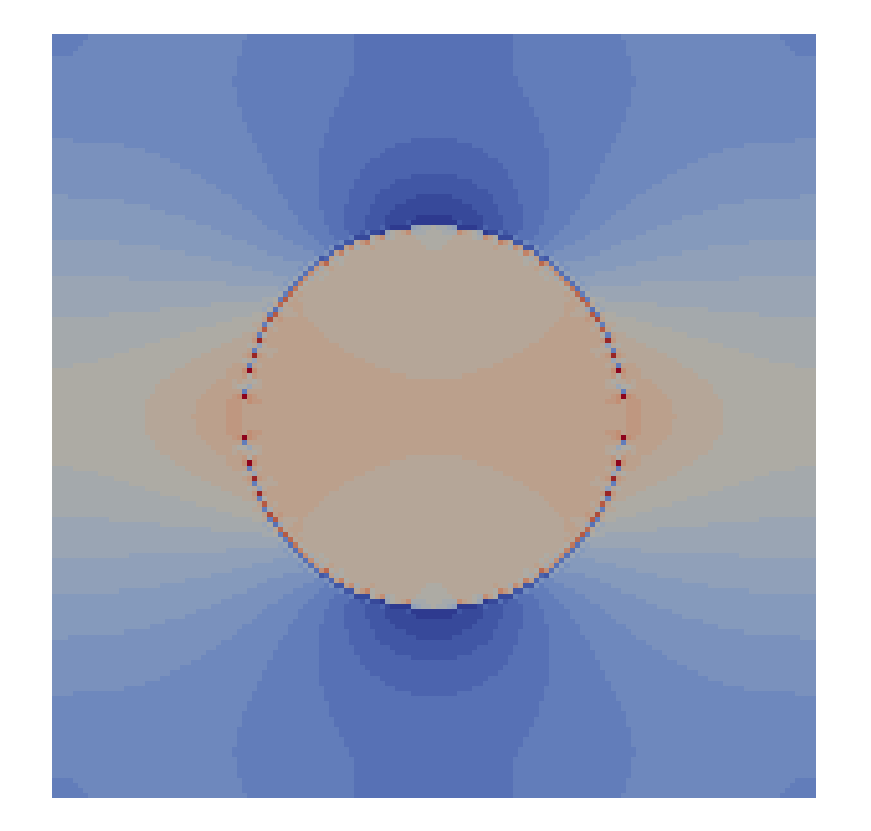
\includegraphics[width=1.1\linewidth]{figures/front_exp_0-crop.pdf}
  \subcaption{\label{fig:front_exp_0}}
\endminipage\hfill
\hspace{0.01\textwidth}
\minipage{0.31\textwidth}
  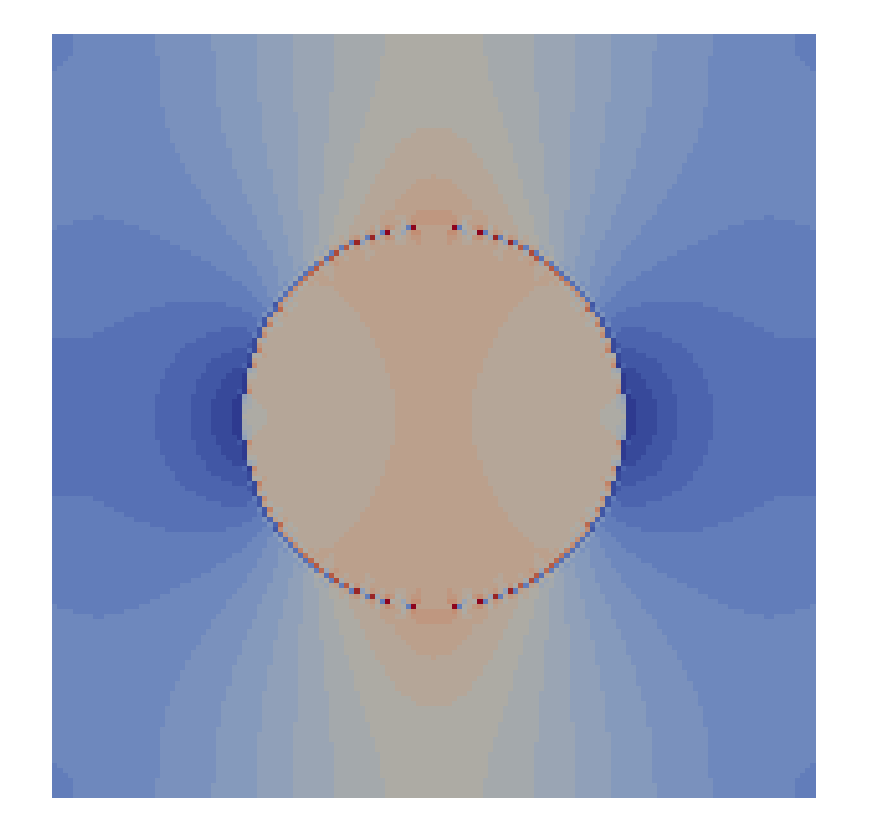
\includegraphics[width=1.1\linewidth]{figures/front_exp_1-crop.pdf}
  \subcaption{\label{fig:front_exp_1}}
\endminipage\hfill
\hspace{0.01\textwidth}
\minipage{0.31\textwidth}%
  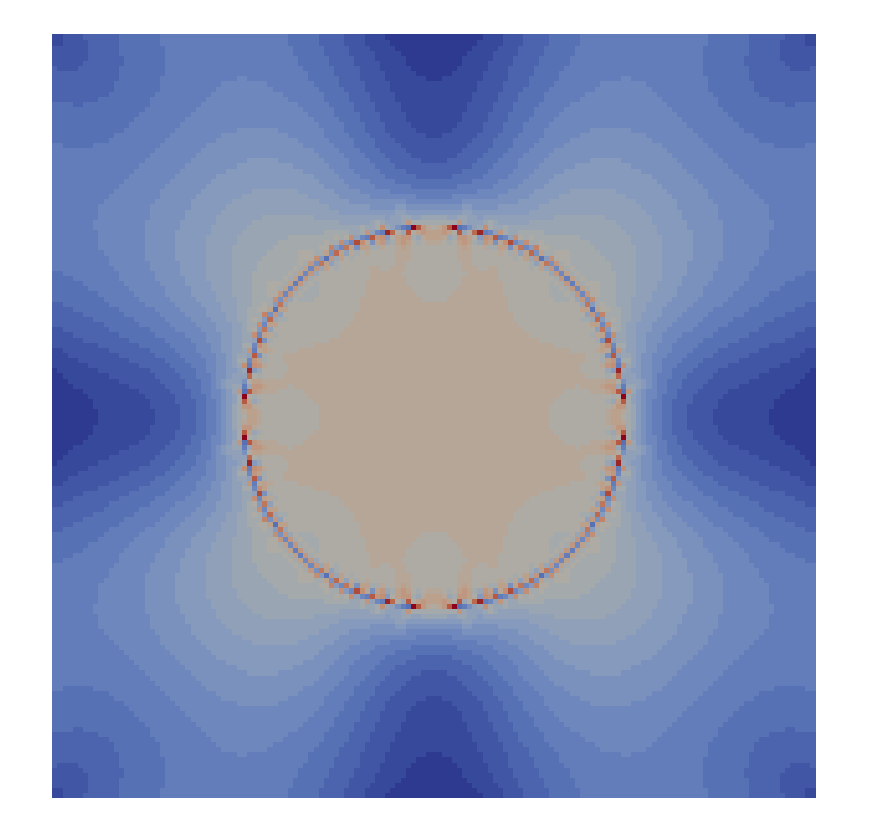
\includegraphics[width=1.1\linewidth]{figures/front_exp_2-crop.pdf}
  \subcaption{\label{fig:front_exp_2}}
\endminipage
\caption{\label{fig:front_exp}}
\end{figure}

\begin{table}[ht]
\centering
\resizebox{1.1\columnwidth}{!}{%
\begin{tabular}{ | S[table-format=1e8,table-column-width=12mm] 
|*4{S[table-format=1.2e4,table-column-width=16mm] }
|*4{S[table-format=1.2e4,table-column-width=16mm] }|}
\hline
{$E_m$} & 
{$\lambda_1^{\text{tp}}$} & 
{$\lambda_1^{\text{ts}}$} & 
{$\lambda_1^{\text{m}}$}  & 
{$\lambda_1^{\text{exact}}$} & 
{$\lambda_2^{\text{tp}}$} & 
{$\lambda_2^{\text{ts}}$} & 
{$\lambda_2^{\text{m}}$}  & 
{$\lambda_2^{\text{exact}}$}\\ 
\hline
2e5 & 2.74e+3 & 9.66e+3 & 9.37e+3 & 9.54e+3 & 4.82e+2 & 1.69e+03 & 1.64e+03 & 1.65e+03\\
5e5 & 1.98e+3 & 3.87e+3 & 3.76e+3 & 3.83e+3 & 3.49e+2 & 6.79e+02 & 6.61e+02 & 6.63e+02\\
8e5 & 1.55e+3 & 2.42e+3 & 2.36e+3 & 2.40e+3 & 2.73e+2 & 4.25e+02 & 4.14e+02 & 4.16e+02\\
1e6 & 1.36e+3 & 1.94e+3 & 1.89e+3 & 1.92e+3 & 2.39e+2 & 3.40e+02 & 3.32e+02 & 3.34e+02\\
2e6 & 8.36e+2 & 9.76e+2 & 9.59e+2 & 9.75e+2 & 1.46e+2 & 1.71e+02 & 1.68e+02 & 1.69e+02\\
5e6 & 3.87e+2 & 3.97e+2 & 3.95e+2 & 4.01e+2 & 6.79e+1 & 6.97e+01 & 6.93e+01 & 6.97e+01\\
8e6 & 2.51e+2 & 2.52e+2 & 2.52e+2 & 2.56e+2 & 4.42e+1 & 4.43e+01 & 4.43e+01 & 4.45e+01\\
1e7 & 2.04e+2 & 2.04e+2 & 2.04e+2 & 2.07e+2 & 3.58e+1 & 3.58e+01 & 3.58e+01 & 3.60e+01\\
2e7 & 1.05e+2 & 1.07e+2 & 1.06e+2 & 1.07e+2 & 1.84e+1 & 1.89e+01 & 1.86e+01 & 1.87e+01\\
5e7 & 4.27e+1 & 4.99e+1 & 4.46e+1 & 4.52e+1 & 7.50e+0 & 8.76e+00 & 7.84e+00 & 7.85e+00\\
8e7 & 2.68e+1 & 3.54e+1 & 2.84e+1 & 2.88e+1 & 4.71e+0 & 6.22e+00 & 4.99e+00 & 4.99e+00\\
1e8 & 2.15e+1 & 3.06e+1 & 2.29e+1 & 2.32e+1 & 3.77e+0 & 5.37e+00 & 4.02e+00 & 4.02e+00\\
2e8 & 1.07e+1 & 2.09e+1 & 1.16e+1 & 1.17e+1 & 1.89e+0 & 3.68e+00 & 2.04e+00 & 2.03e+00\\
\hline 
\end{tabular}
}
\end{table}

%---------------------------------------------------------------------------------------------------

\subsection{Transversal fibers}

\begin{figure}[!ht]
\begin{minipage}[b]{0.47\linewidth}
\subcaptionbox{\label{fig:geo2_geom}}{
\resizebox{6.2cm}{!}{\documentclass{standalone}

\begin{document}

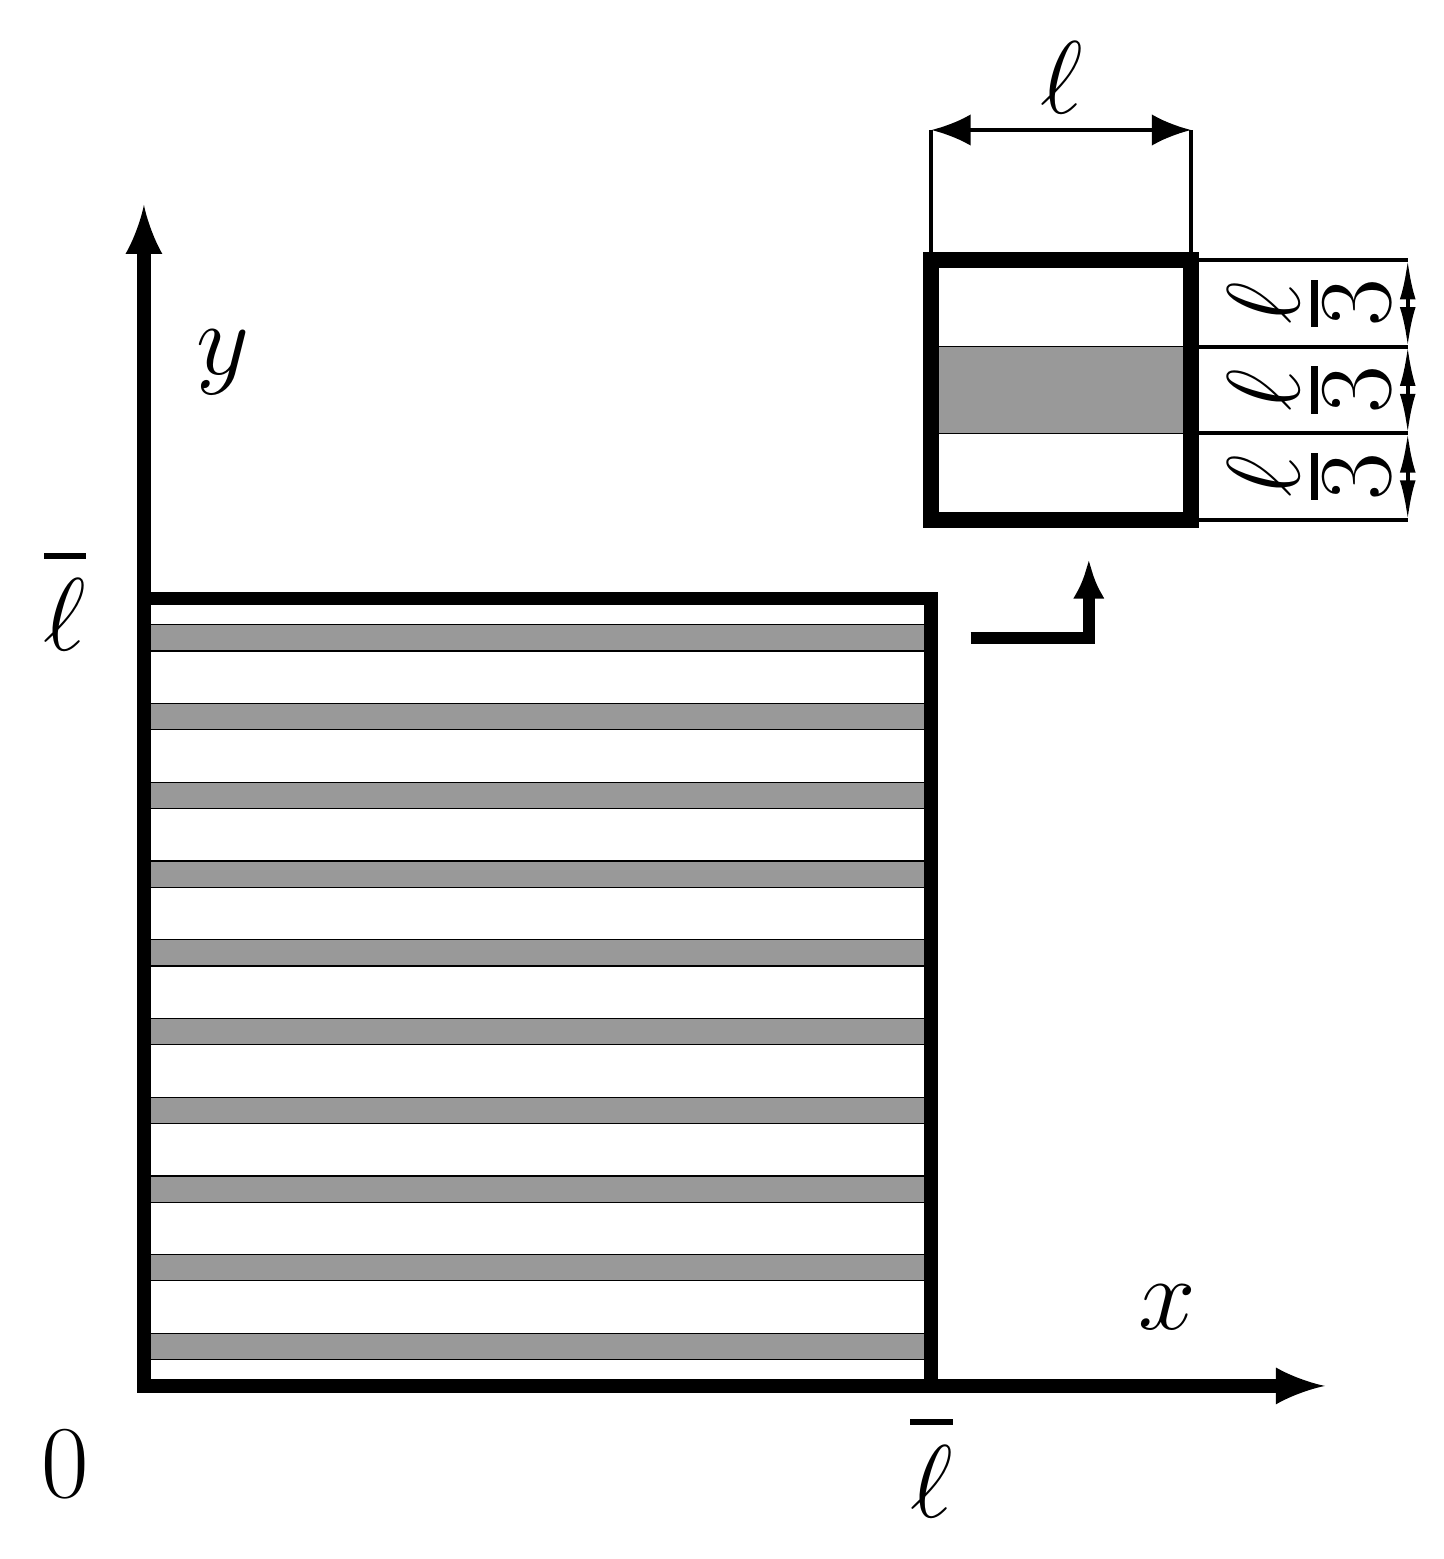
\begin{tikzpicture}[>=latex,node distance=0pt,font={\fontsize{40pt}{12}\selectfont}]

% structure
\foreach \y [count=\n]in {0,1,2,3,4,5,6,7,8,9}
{
  \def\j{\y*1.0};
  \begin{scope}[yshift = \j cm,xshift = 0 cm,start chain=going right]
   \filldraw[fill=black!40!white,draw=black] (0,0.3333) -- (10,0.3333) -- (10,0.6666) -- (0,0.6666) -- cycle;
  \end{scope}
}
\draw[line width=1.75mm] (0,0) -- (10,0) -- (10,10) -- (0,10) -- cycle;




\draw[-{Latex[length=5mm,width=4mm]}, line width=1.5mm] (10.5,9.5) -- ++(1.5,0)
  -- ++(0,1);

% rve
\begin{scope}[xshift=10.0cm,yshift=11cm, rotate=0.0, scale=1.1]

 \filldraw[fill=black!40!white,draw=black] (0,1) rectangle (3,2);
 \draw[draw=black, line width=2.0mm] (0,0) rectangle (3,3);

 \draw[line width=0.5mm] (3,0) -- ++(2.5,0);
 \draw[line width=0.5mm] (3,1) -- ++(2.5,0);
 \draw[line width=0.5mm] (3,2) -- ++(2.5,0);
 \draw[line width=0.5mm] (3,3) -- ++(2.5,0);

 \draw[{Latex[length=5mm,width=2mm]}-{Latex[length=5mm,width=2mm]},line width=0.5mm]
 (5.5,1) --  node[above,rotate=90,scale=1.5] {$\frac{\ell}{3}$}  ++(0,1);
 \draw[{Latex[length=5mm,width=2mm]}-{Latex[length=5mm,width=2mm]},line width=0.5mm]
 (5.5,2) --  node[above,rotate=90,scale=1.5] {$\frac{\ell}{3}$}  ++(0,1);
 \draw[{Latex[length=5mm,width=2mm]}-{Latex[length=5mm,width=2mm]},line width=0.5mm]
 (5.5,0) --  node[above,rotate=90,scale=1.5] {$\frac{\ell}{3}$}  ++(0,1);

 \draw[line width=0.5mm] (0,3) -- ++(0,1.5);
 \draw[line width=0.5mm] (3,3) -- ++(0,1.5);
 \draw[{Latex[length=5mm,width=4mm]}-{Latex[length=5mm,width=4mm]},line width=0.5mm] 
 (0,4.5) --  node[above,scale=1.5] {$\ell$}  ++(3,0);

\end{scope}

% axes
\draw[-latex,line width=1.75mm] (0,10) -- ++ (0, 5) ;
\draw[-latex,line width=1.75mm] (10,0) -- ++ (5, 0) ;
\node[scale=1.5] (a) at (13,1)  {$x$};
\node[scale=1.5] (a) at (1,13)  {$y$};
\node[scale=1.5] (a) at (-1,-1) {$0$};
\node[scale=1.5] (a) at (10,-1) {$\overline{\ell}$};
\node[scale=1.5] (a) at (-1,10) {$\overline{\ell}$};

\end{tikzpicture}

\end{document}
}}
\end{minipage}
\hspace{1.5cm}
\begin{minipage}[b]{0.47\linewidth}
\subcaptionbox{\label{fig:geo2_geom}}{
\resizebox{6cm}{!}{\documentclass{standalone}

\begin{document}

\begin{tikzpicture}[>=latex,node distance=0pt,font={\fontsize{40pt}{12}\selectfont}]

    \draw[step=1cm,black] (0,0) grid (10,10);
    \node[inner sep=0pt, scale=0.5] (rve) at (12,12.5)
        {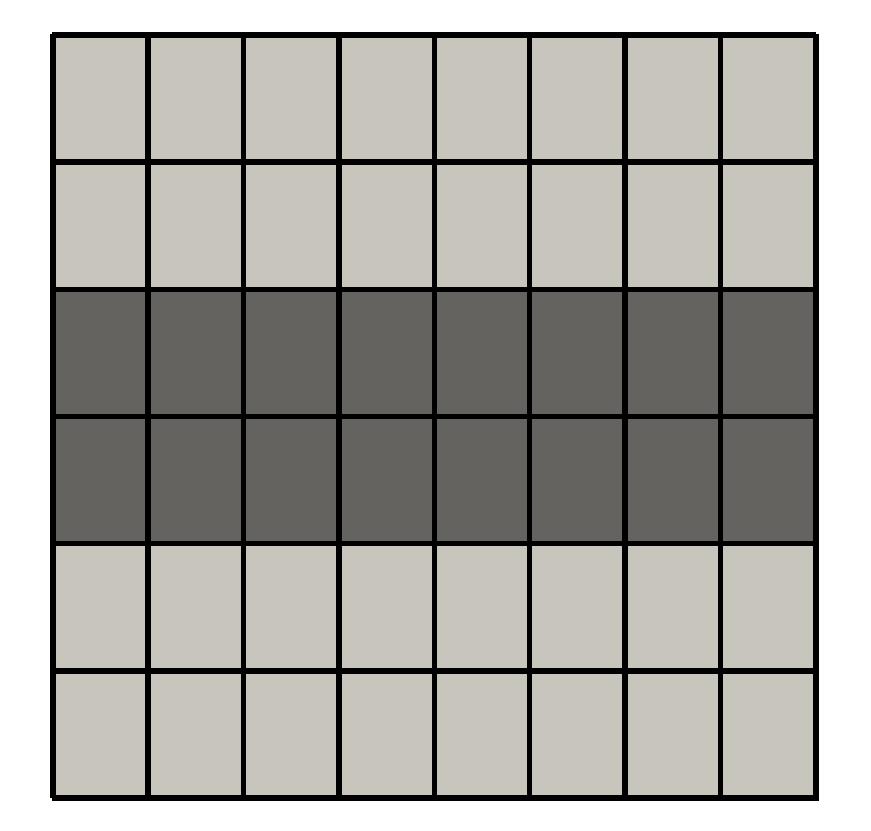
\includegraphics[width=1.4\textwidth]{figures/direct_mesh_transversal_zoom-crop.pdf}};
    \draw[draw=black, line width=2.0mm] (9,9) rectangle (10,10);
    \draw[-{Latex[length=5mm,width=4mm]}, line width=1.5mm] (10.5,9.5) -- ++(1.5,0) -- ++(0,1);

    % axes
    \draw[-latex,line width=1.75mm] (0,0) -- ++ (0, 15) ;
    \draw[-latex,line width=1.75mm] (0,0) -- ++ (15, 0) ;
    \node[scale=1.5] (a) at (13,1) {$x$};
    \node[scale=1.5] (a) at (1,13) {$y$};
    \node[scale=1.5] (a) at (-1,-1) {$0$};
    \node[scale=1.5] (a) at (10,-1) {$\overline{\ell}$};
    \node[scale=1.5] (a) at (-1,10) {$\overline{\ell}$};

\end{tikzpicture}

\end{document}
}}
\end{minipage}
\caption{\emph{Transversal fiber} example.}
\label{fig_dist_scheme}
\end{figure}

\subsubsection{Homogenization model}

\begin{figure}[!ht]
\centering
\resizebox{5.0cm}{!}{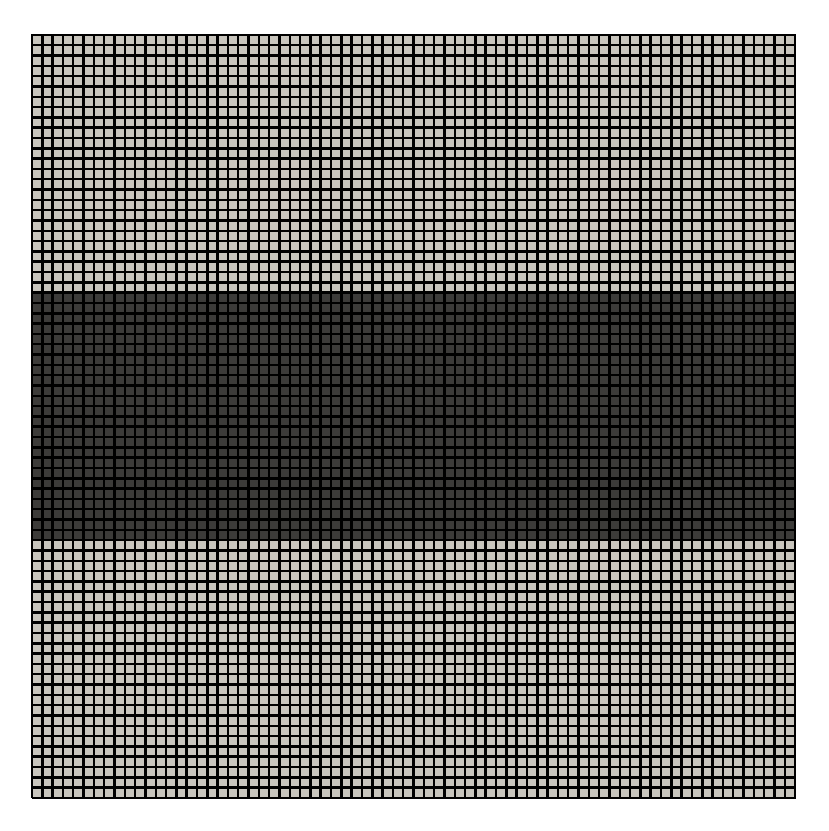
\includegraphics[width=1.4\textwidth]{figures/rve_6_msh-crop.pdf}}
\caption{Representative volume element to perform the homogenization calculation for obtaining the 
average properties $\overline{\bm{\sigma}}$ and $\overline{\mathbb{C}}$.}
\label{fig_rve_front_fib}
\end{figure}

\begin{equation}
\overline{\mathbb{C}}_h = 
  \begin{bmatrix}
   \begin{tabular}{ @{}*{3}{S[round-mode=places,
                    round-integer-to-decimal,round-precision=2,
                    table-format=1.2e4,table-column-width=16mm,table-number-alignment=center]}@{}
		  }
    4.705669e+06 & 9.313840e+05 & 0.0          \\
    9.313840e+05 & 2.173229e+06 & 0.0          \\
    0.0          & 0.0          & 7.953203e+05
   \end{tabular}
  \end{bmatrix}
\end{equation}

\begin{equation}
\overline{\mathbb{C}}_p = 
  \begin{bmatrix}
   \begin{tabular}{ @{}*{3}{S[round-mode=places,
                    round-integer-to-decimal,round-precision=2,
                    table-format=1.2e4,table-column-width=16mm,table-number-alignment=center]}@{}
		  }
   5.275468e+06 & 2.260915e+06 & 0.0          \\
   2.260915e+06 & 5.275468e+06 & 0.0          \\
   0.0          & 0.0          & 1.507277e+06
  \end{tabular}
  \end{bmatrix}
\end{equation}

\begin{equation}
  \overline{\mathbb{C}}_s = 
  \begin{bmatrix}
   \begin{tabular}{ @{}*{3}{S[round-mode=places,
                    round-integer-to-decimal,round-precision=2,
                    table-format=1.2e4,table-column-width=16mm,table-number-alignment=center]}@{}
		  }
    1.901057e+06 & 8.147387e+05 & 0.0          \\
    8.147387e+05 & 1.901057e+06 & 0.0          \\
    0.0          & 0.0          & 5.431591e+05
   \end{tabular}
  \end{bmatrix}
\end{equation}

\begin{figure}[!ht]
\begin{minipage}[b]{0.4\linewidth}
 \resizebox{7.0cm}{!}
 {
  \begin{tikzpicture}
   \pgfplotstableread{data/trans_fiber/direct.dat}{\direct}
   \pgfplotstableread{data/trans_fiber/homog_us.dat}{\homogus}
   \pgfplotstableread{data/trans_fiber/homog_tp.dat}{\homogtp}
   \pgfplotstableread{data/trans_fiber/homog_ts.dat}{\homogts}
   \begin{axis}[
     xlabel=$d$,ylabel=$f$,
     ymax=50000,
     tick scale binop=\times,
     scaled y ticks={base 10:-4},
     tick label style={/pgf/number format/fixed},
     grid=both,
     legend pos=north west
   ]
   \addplot+[line width=2pt,mark=+,mark options={scale=3},color=black] table [x index=0, y index=2] {\direct};\addlegendentry{DIRECT};
   \addplot+[mark=*,mark options={scale=0.5},color=blue]               table [x index=0, y index=2] {\homogus};\addlegendentry{FE$^2$-US};
   \addplot+[mark=*,mark options={scale=0.5},color=red]                table [x index=0, y index=2] {\homogtp};\addlegendentry{MIX-P};
   \addplot+[mark=*,mark options={scale=0.5},color=green]              table [x index=0, y index=2] {\homogts};\addlegendentry{MIX-S};
   \end{axis}
  \end{tikzpicture}
 }
\end{minipage}
\hspace{3cm}
\begin{minipage}[b]{0.4\linewidth}
 \resizebox{7.0cm}{!}
 {
  \begin{tikzpicture}
   \pgfplotstableread{data/trans_fiber/direct.dat}{\direct}
   \pgfplotstableread{data/trans_fiber/homog_us.dat}{\homogus}
   \pgfplotstableread{data/trans_fiber/homog_tp.dat}{\homogtp}
   \pgfplotstableread{data/trans_fiber/homog_ts.dat}{\homogts}
   \begin{axis}[
     xlabel=$d$,ylabel=$f$,
     ymax=12000,
     tick scale binop=\times,
     scaled y ticks={base 10:-4},
     tick label style={/pgf/number format/fixed},
     grid=both,
     legend pos=north west
   ]
   \addplot+[line width=2pt,mark=+,mark options={scale=3},color=black] table [x index=0, y index=3] {\direct};\addlegendentry{DIRECT};
   \addplot+[mark=*,mark options={scale=0.5},color=blue]               table [x index=0, y index=3] {\homogus};\addlegendentry{FE$^2$-US};
   \addplot+[mark=*,mark options={scale=0.5},color=red]                table [x index=0, y index=3] {\homogtp};\addlegendentry{MIX-P};
   \addplot+[mark=*,mark options={scale=0.5},color=green]              table [x index=0, y index=3] {\homogts};\addlegendentry{MIX-S};
   \end{axis}
  \end{tikzpicture}
 }
\end{minipage}
\end{figure}

\begin{figure}[!ht]
\begin{minipage}[b]{0.4\linewidth}
 \resizebox{7.0cm}{!}
 {
  \begin{tikzpicture}
   \pgfplotstableread{data/trans_fiber/omega_direct_0.dat}{\direct}
   \pgfplotstableread{data/trans_fiber/omega_us_0.dat}{\homogus}
   \pgfplotstableread{data/trans_fiber/omega_tp_0.dat}{\homogtp}
   \pgfplotstableread{data/trans_fiber/omega_ts_0.dat}{\homogts}
   \begin{axis}[
     xlabel=$d$,ylabel=$\lambda_0$,
     xmode = log,
     ymax=12000,
     tick scale binop=\times,
     scaled y ticks={base 10:-3},
     y tick label style={/pgf/number format/.cd, fixed zerofill, 1000 sep={}, precision=1, /tikz/.cd},
     grid=both,
     legend pos=north east
   ]
   \addplot+[line width=2pt,mark=+,mark options={scale=3},color=black] table [x index=0, y index=1] {\direct};\addlegendentry{DIRECT};
   \addplot+[mark=*,mark options={scale=0.5},color=blue]               table [x index=0, y index=1] {\homogus};\addlegendentry{FE$^2$-US};
   \addplot+[mark=*,mark options={scale=0.5},color=red]                table [x index=0, y index=1] {\homogtp};\addlegendentry{MIX-P};
   \addplot+[mark=*,mark options={scale=0.5},color=green]              table [x index=0, y index=1] {\homogts};\addlegendentry{MIX-S};
   \end{axis}
  \end{tikzpicture}
 }
\end{minipage}
\hspace{3cm}
\begin{minipage}[b]{0.4\linewidth}
 \resizebox{7.0cm}{!}
 {
  \begin{tikzpicture}
   \pgfplotstableread{data/trans_fiber/omega_direct_1.dat}{\direct}
   \pgfplotstableread{data/trans_fiber/omega_us_1.dat}{\homogus}
   \pgfplotstableread{data/trans_fiber/omega_tp_1.dat}{\homogtp}
   \pgfplotstableread{data/trans_fiber/omega_ts_1.dat}{\homogts}
   \begin{axis}[
     xlabel=$d$,ylabel=$\lambda_1$,
     xmode = log,
     ymax=4000,
     tick scale binop=\times,
     scaled y ticks={base 10:-3},
     y tick label style={/pgf/number format/.cd, fixed zerofill, 1000 sep={}, precision=1, /tikz/.cd},
     grid = both,
     legend pos = north east
   ]
   \addplot+[line width=2pt,mark=+,mark options={scale=3},color=black] table [x index=0, y index=1] {\direct};\addlegendentry{DIRECT};
   \addplot+[mark=*,mark options={scale=0.5},color=blue]               table [x index=0, y index=1] {\homogus};\addlegendentry{FE$^2$-US};
   \addplot+[mark=*,mark options={scale=0.5},color=red]                table [x index=0, y index=1] {\homogtp};\addlegendentry{MIX-P};
   \addplot+[mark=*,mark options={scale=0.5},color=green]              table [x index=0, y index=1] {\homogts};\addlegendentry{MIX-S};
   \end{axis}
  \end{tikzpicture}
 }
\end{minipage}
\end{figure}

\begin{table}[ht]
\centering
\resizebox{1.1\columnwidth}{!}{%
\begin{tabular}{ | S[table-format=1e8,table-column-width=12mm] 
|*4{S[table-format=1.2e4,table-column-width=16mm] }
|*4{S[table-format=1.2e4,table-column-width=16mm] }|}
\hline
{$E_m$} & 
{$\lambda_1^{\text{tp}}$}    & 
{$\lambda_1^{\text{ts}}$}    & 
{$\lambda_1^{\text{m}}$}     & 
{$\lambda_1^{\text{exact}}$} & 
{$\lambda_2^{\text{tp}}$}    & 

{$\lambda_2^{\text{ts}}$}    & 
{$\lambda_2^{\text{m}}$}     & 
{$\lambda_2^{\text{exact}}$}\\ 
\hline
2e5 & 5.89e+2 & 6.88e+3 & 1.26e+3 & 3.51e+3 & 1.03e+2 & 1.20e+3 & 1.50e+2 & 3.73e+2\\
5e5 & 5.57e+2 & 2.79e+3 & 9.73e+2 & 1.64e+3 & 9.78e+1 & 4.90e+2 & 1.21e+2 & 1.86e+2\\
8e5 & 5.28e+2 & 1.77e+3 & 8.10e+2 & 1.14e+3 & 9.27e+1 & 3.10e+2 & 1.04e+2 & 1.36e+2\\
1e6 & 5.10e+2 & 1.43e+3 & 7.35e+2 & 9.68e+2 & 8.96e+1 & 2.51e+2 & 9.61e+1 & 1.18e+2\\
2e6 & 4.37e+2 & 7.49e+2 & 5.27e+2 & 5.97e+2 & 7.68e+1 & 1.31e+2 & 7.76e+1 & 7.96e+1\\
5e6 & 3.06e+2 & 3.40e+2 & 3.17e+2 & 3.28e+2 & 5.38e+1 & 5.97e+1 & 5.39e+1 & 5.42e+1\\
8e6 & 2.35e+2 & 2.38e+2 & 2.36e+2 & 2.41e+2 & 4.13e+1 & 4.18e+1 & 4.14e+1 & 4.16e+1\\
1e7 & 2.04e+2 & 2.04e+2 & 2.04e+2 & 2.07e+2 & 3.58e+1 & 3.58e+1 & 3.58e+1 & 3.60e+1\\
2e7 & 1.22e+2 & 1.36e+2 & 1.26e+2 & 1.30e+2 & 2.15e+1 & 2.39e+1 & 2.15e+1 & 2.16e+1\\
5e7 & 5.57e+1 & 9.53e+1 & 6.31e+1 & 7.47e+1 & 9.78e+0 & 1.67e+1 & 9.86e+0 & 9.94e+0\\
8e7 & 3.60e+1 & 8.51e+1 & 4.31e+1 & 5.89e+1 & 6.33e+0 & 1.49e+1 & 6.40e+0 & 7.36e+0\\
1e8 & 2.91e+1 & 8.17e+1 & 3.58e+1 & 5.33e+1 & 5.12e+0 & 1.43e+1 & 5.19e+0 & 6.44e+0\\
2e8 & 1.49e+1 & 7.49e+1 & 1.95e+1 & 4.13e+1 & 2.62e+0 & 1.31e+1 & 2.67e+0 & 4.49e+0\\
5e8 & 6.07e+0 & 7.08e+1 & 8.33e+0 & 3.20e+1 & 1.06e+0 & 1.24e+1 & 1.10e+0 & 3.13e+0\\
\hline 
\end{tabular}
}
\end{table}

%---------------------------------------------------------------------------------------------------
\section{Conclusions}

%---------------------------------------------------------------------------------------------------
\newpage
\newpage
\section*{References}

\bibliography{../mybibfile}

\end{document}
